\section{Summary of Requested Beam Time Allocations}
\paragraph{}
An experiment is proposed to measure the longitudinal virtual photon asymmetries $A_1^{n,h}$ in the SIDIS reaction on a longitudinally polarized $^3$He target. The experiment will use a high-luminosity polarized $^3$He target currently under development for several approved experiments, together with the BigBite~\cite{BigBiteOptics1998,BigBite1998,BigBiteOptics2012} and Super BigBite~\cite{SBS_CDR,SBS_CDR_NEW} spectrometers in Hall A. There are essentially five adjustable parameters of the experiment; the beam energy $E_{beam}$, the two spectrometer angles $\theta_{BB}$ and $\theta_{SBS}$, and the target-magnet yoke distances $d_{BB}$ and $d_{SBS}$.
\begin{table}[h]
  \begin{center}
    \caption{\label{Kintable} Requested beam time allocations. In total, 30 beam-days of production on $^3$He and 3 beam-days for configuration changes and calibration measurements are requested. Production data collection is divided between beam energies of 11 GeV (20 days) and 8.8 GeV (10 days). At each beam energy, the beam time is divided equally between two SBS angle settings of 14 and 10 degrees. Calibrations include measurements on unpolarized $^3$He, N$_2$, H$_2$ and empty reference cells for dilutions and multi-foil solid targets for spectrometer optics calibrations. $E_{beam}$ is the beam energy, $\theta_{BB/SBS}$ is the spectrometer central angle and $d_{BB/SBS}$ is the distance from the center of the target to the front face of the magnet yoke along the spectrometer axis.}
    \begin{tabular}{ccccccc}
      \hline \hline Beam days & Purpose & $E_{beam}$ (GeV) & $\theta_{BB}$ (deg.) & $\theta_{SBS}$ (deg.) & $d_{BB}$ (m) & $d_{SBS}$ (m)  \\ \hline 
      10 & Production & 11 & 30 & 14 & 1.55 & 2.5 \\ 
      10 & Production & 11 & 30 & 10 & 1.55 & 2.6 \\
      5 & Production & 8.8 & 30 & 14 & 1.55 & 2.5  \\ 
      5 & Production & 8.8 & 30 & 10 & 1.55 & 2.6  \\
      1 & Calibration & 11 & 30 & 14 & 1.55 & 2.5  \\
      1 & Calibration & 11 & 30 & 10 & 1.55 & 2.6 \\
      0.5 & Calibration & 8.8 & 30 & 14 & 1.55 & 2.5 \\ 
      0.5 & Calibration & 8.8 & 30 & 10 & 1.55 & 2.6  \\ \hline 
      30 & Total production & & & & &  \\ 
      3 & Total calibrations & & & & &  \\ \hline \hline
    \end{tabular}
  \end{center}
\end{table}
Table~\ref{Kintable} shows the requested beam allocations in each experiment configuration. The configuration of the spectrometers in the proposed experiment is identical to that of the approved experiment E12-09-018~\cite{SBS_SIDIS} in most respects. The main differences between the proposed experiment and E12-09-018 are: 
\begin{itemize}
\item This proposal uses a longitudinally polarized $^3$He target, whereas E12-09-018 will measure asymmetries on a transversely polarized target. 
\item The proposed experiment also includes data taking at a smaller SBS central angle of 10$^\circ$ to focus the hadron arm acceptance at smaller values of $p_T^h$, where the $\phi_h$ coverage is more complete and SIDIS cross sections are larger. 
\end{itemize}
The double-spin asymmetries will be extracted with high statistical precision in a dense two-dimensional grid of $(x,z)$ for $\pi^{\pm,0}$ and $K^\pm$, with $0.1 \le x \le 0.7$ and $0.2 \le z \le 0.8$. The data from two different SBS central angles will also provide a wide coverage in $p_T^h$ and $\phi_h$ at the same $x$ and $z$. Data at two different beam energies provide significantly different $Q^2$ values at the same $x$, leading to a ``fully differential'' mapping of the SIDIS asymmetries. However, since the main physics goal of this proposal is to provide data of high statistical precision for the flavor decomposition of the nucleon's longitudinal spin structure in the collinear approximation, the two-dimensional $(x,z)$ kinematic binning is emphasized in this proposal.

\begin{figure}[h]
  \begin{center}
    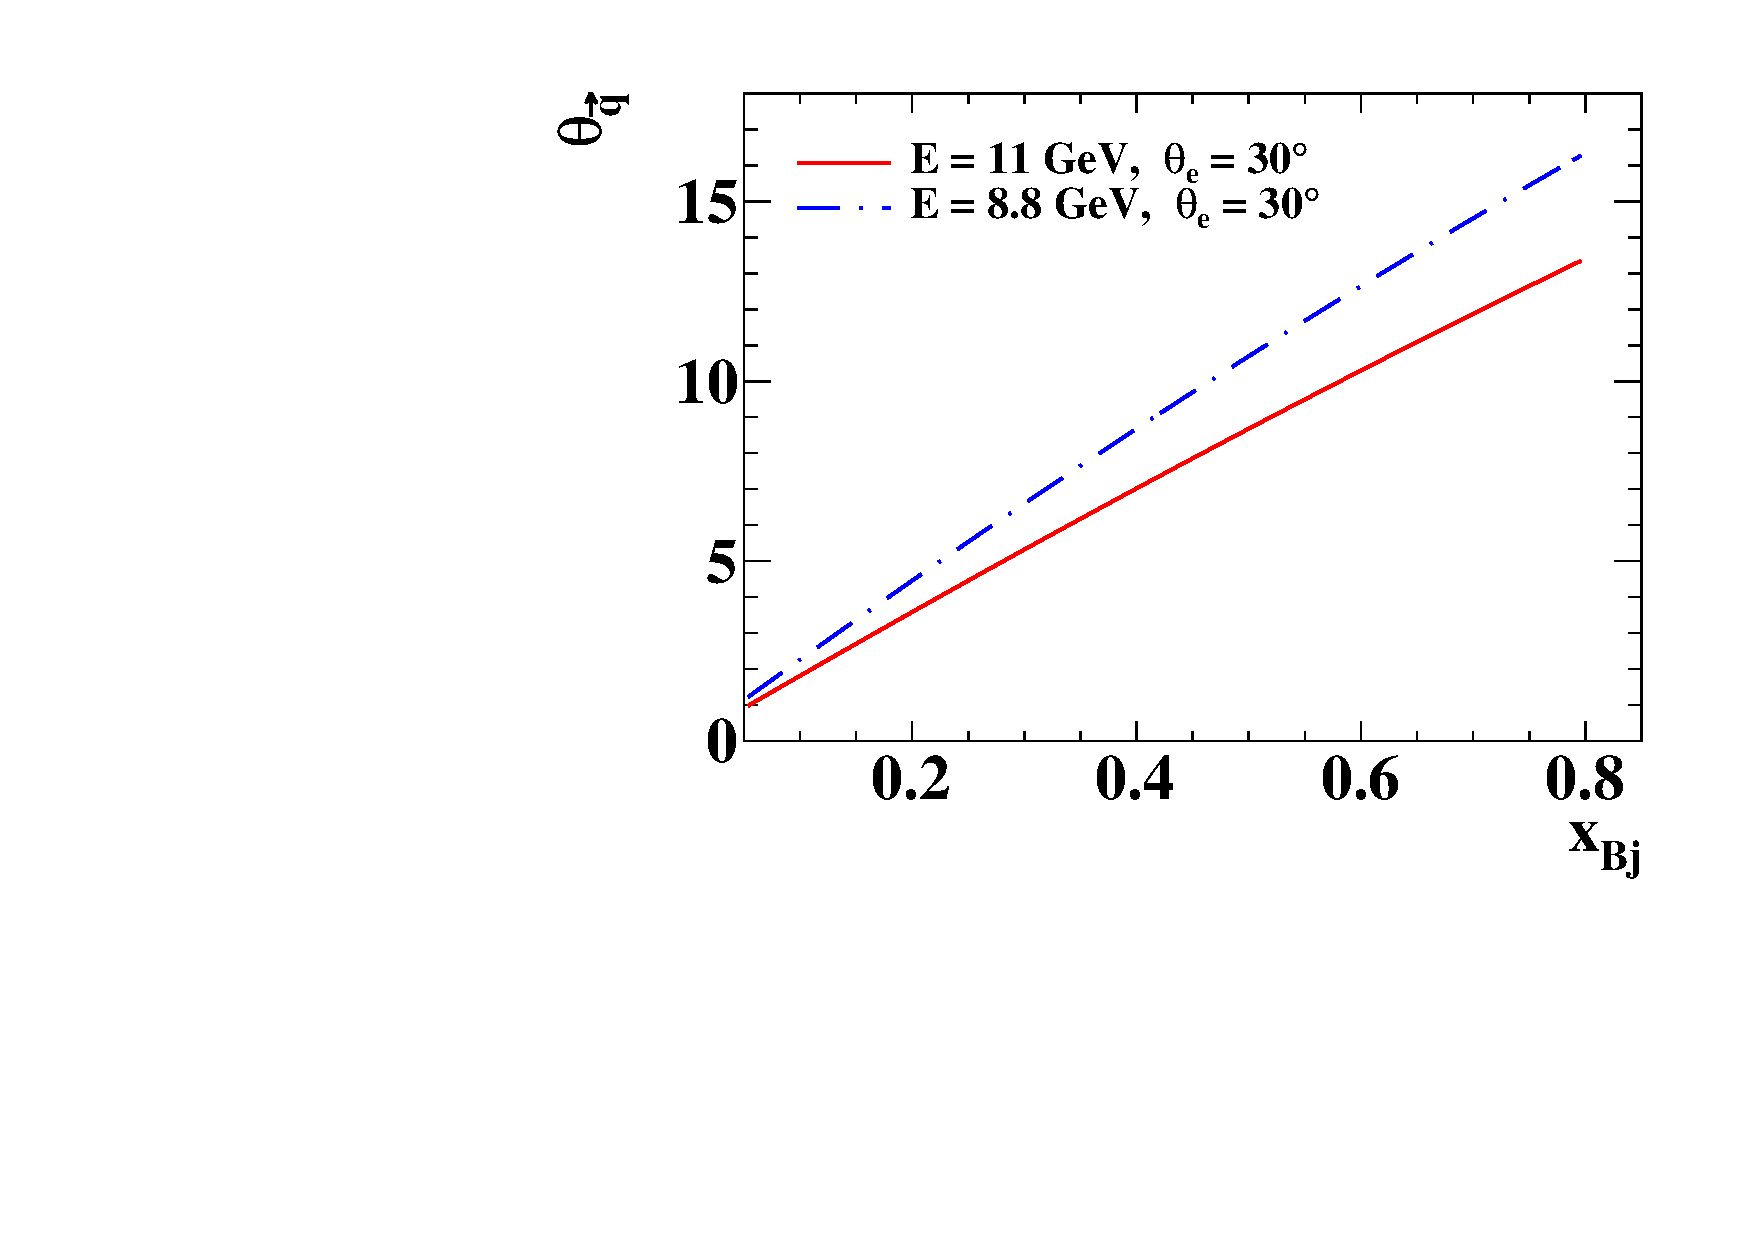
\includegraphics[width=0.48\textwidth]{figures/thqxfig.pdf}
    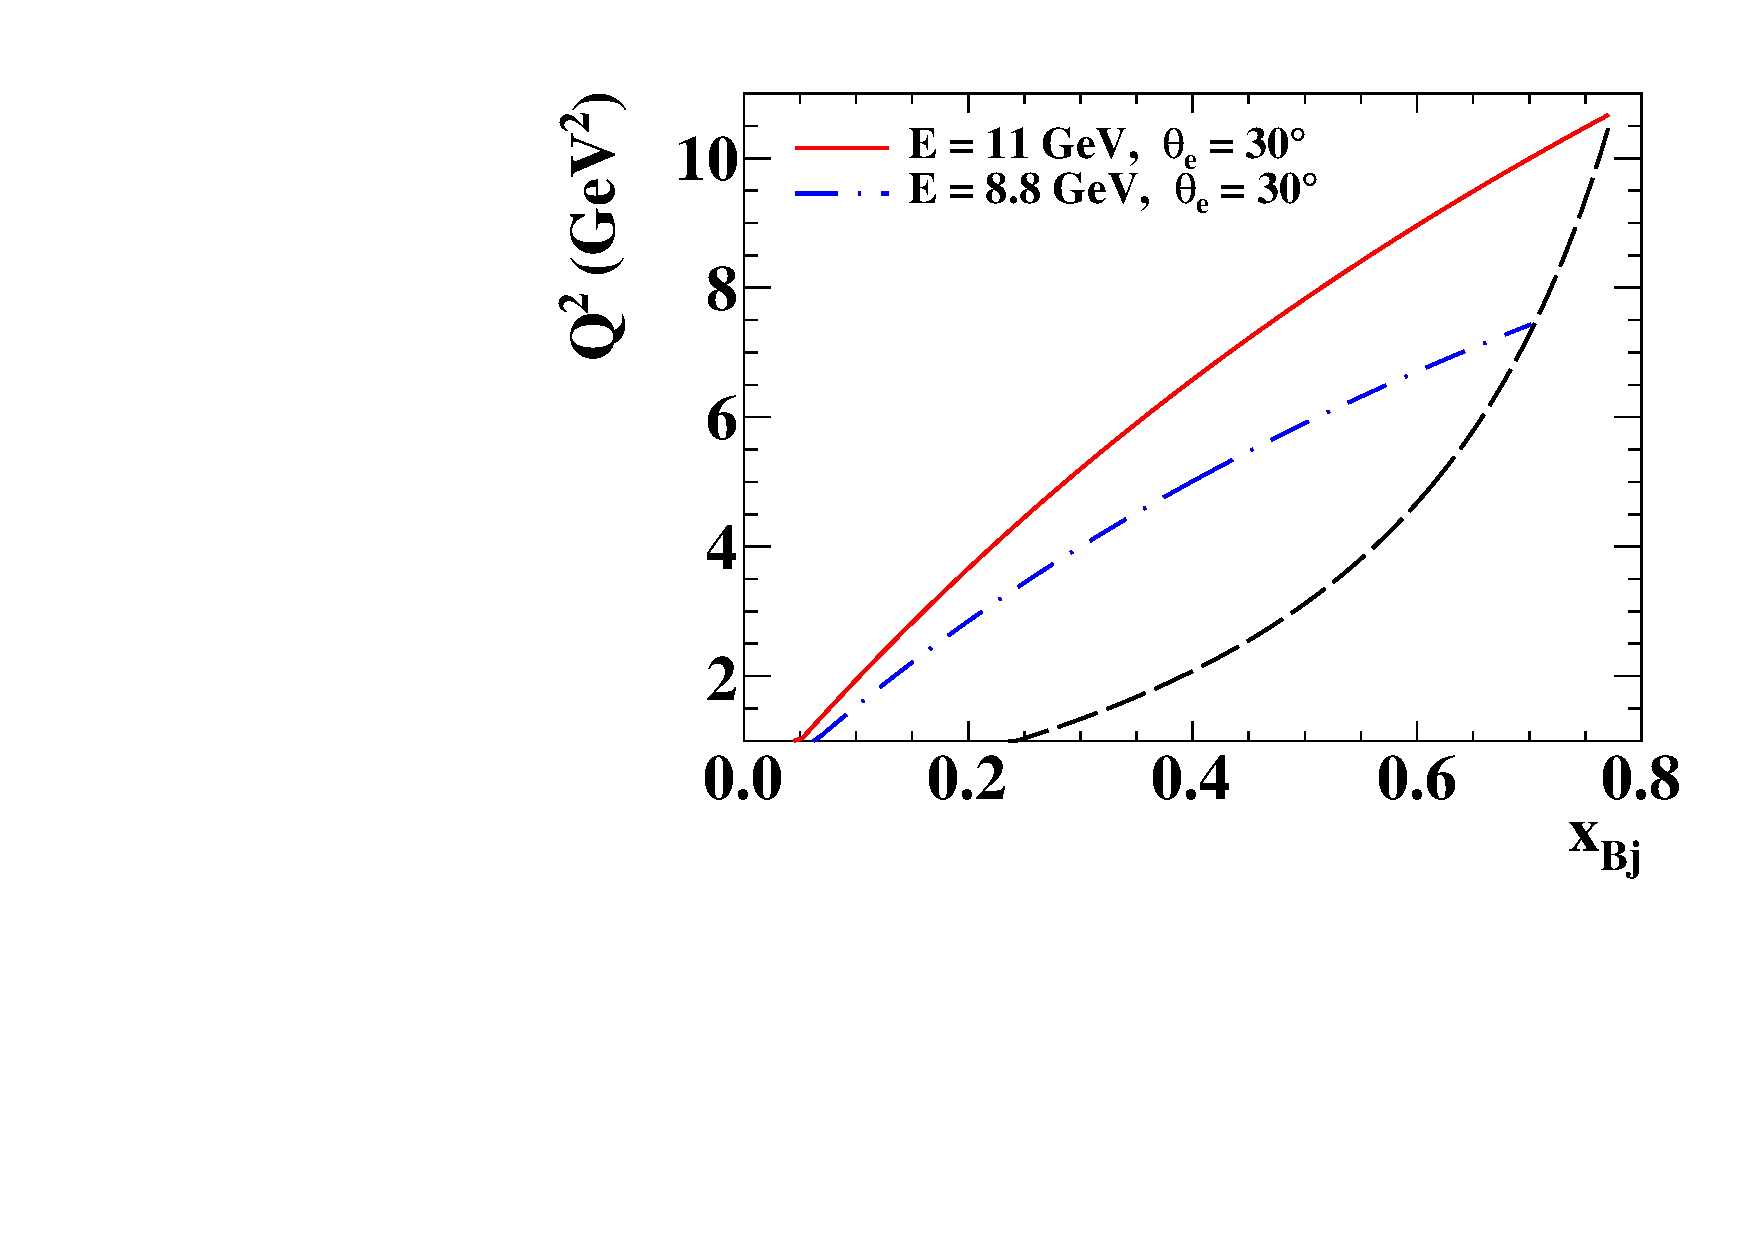
\includegraphics[width=0.48\textwidth]{figures/Q2xfig.pdf}
  \end{center}
  \caption{\label{fig:thqx} Left: Angle of the momentum transfer $\vec{q}$ relative to the beam direction vs $x$ for an electron scattering angle $\theta_e = 30^\circ $ and beam energies of 11 and 8.8 GeV. Right: $Q^2$ vs $x$ at $\theta_e = 30^\circ$ for 11 and 8.8 GeV. The black dashed curve shows the $W > 2$ GeV cutoff.}
\end{figure}
The motivation for taking roughly half the data at a smaller SBS central angle derives from the differences in physics goals between this proposal and E12-09-018. Figure~\ref{fig:thqx} shows the direction of the momentum transfer $\vec{q}$ as a function of $x$ at the central electron scattering angle of 30 degrees. In the absence of competing constraints, the optimal hadron arm angle coincides with the virtual photon direction $\theta_{\vec{q}}$. Since $\theta_{\vec{q}}$ varies as a function of $x$, the hadron arm acceptance can only be centered along $\vec{q}$ for a particular value of $x$. The transverse target single-spin asymmetries that will be measured by E12-09-018 vanish as $p_T^h \rightarrow 0$, such that the optimal SBS central angle is that which centers the SIDIS kinematic coverage at moderate, non-zero $p_T^h$. On the other hand, the longitudinal double-spin asymmetries used as input to the extraction of flavor-separated quark helicity distributions $\Delta q$ do not vanish as $p_T^h \rightarrow 0$, so the optimal central angle of the hadron arm in this experiment is that which maximizes the SIDIS event rate for the $x-Q^2$ range covered by the electron arm. The potential benefit of moving to smaller SBS central angles is limited by the spatial constraints of the BigBite and SBS magnet and detector geometries and the downstream beam pipe in Hall A; for a fixed position of BigBite, the minimum target-SBS magnet distance increases as the SBS central angle is reduced. Moreover, the detector background rates increase at smaller angles. The data obtained at two different SBS central angles will result in an overall increase in $\phi_h$ and $p_T^h$ coverage and a significant increase in total statistics at lower $x$ and $p_T^h$ values. 
\section{Experiment Apparatus}
\paragraph{}
In the proposed experiment, longitudinally polarized electron beams from CEBAF with energies of 11 and 8.8 GeV will collide with longitudinally polarized $^3$He nuclei in a 60 cm-long target. A beam polarization of 85\% is assumed throughout this proposal. This value for electron beam polarization has been routinely achieved and exceeded during the 6 GeV era of CEBAF operations. The beam current will be 40 $\mu$A on the 60-cm target at a pressure of 10.5 atm, leading to an effective electron-polarized-neutron luminosity of approximately $4\times 10^{36}$ cm$^{-2}$ s$^{-1}$. 
\begin{figure}[h]
  \begin{center}
    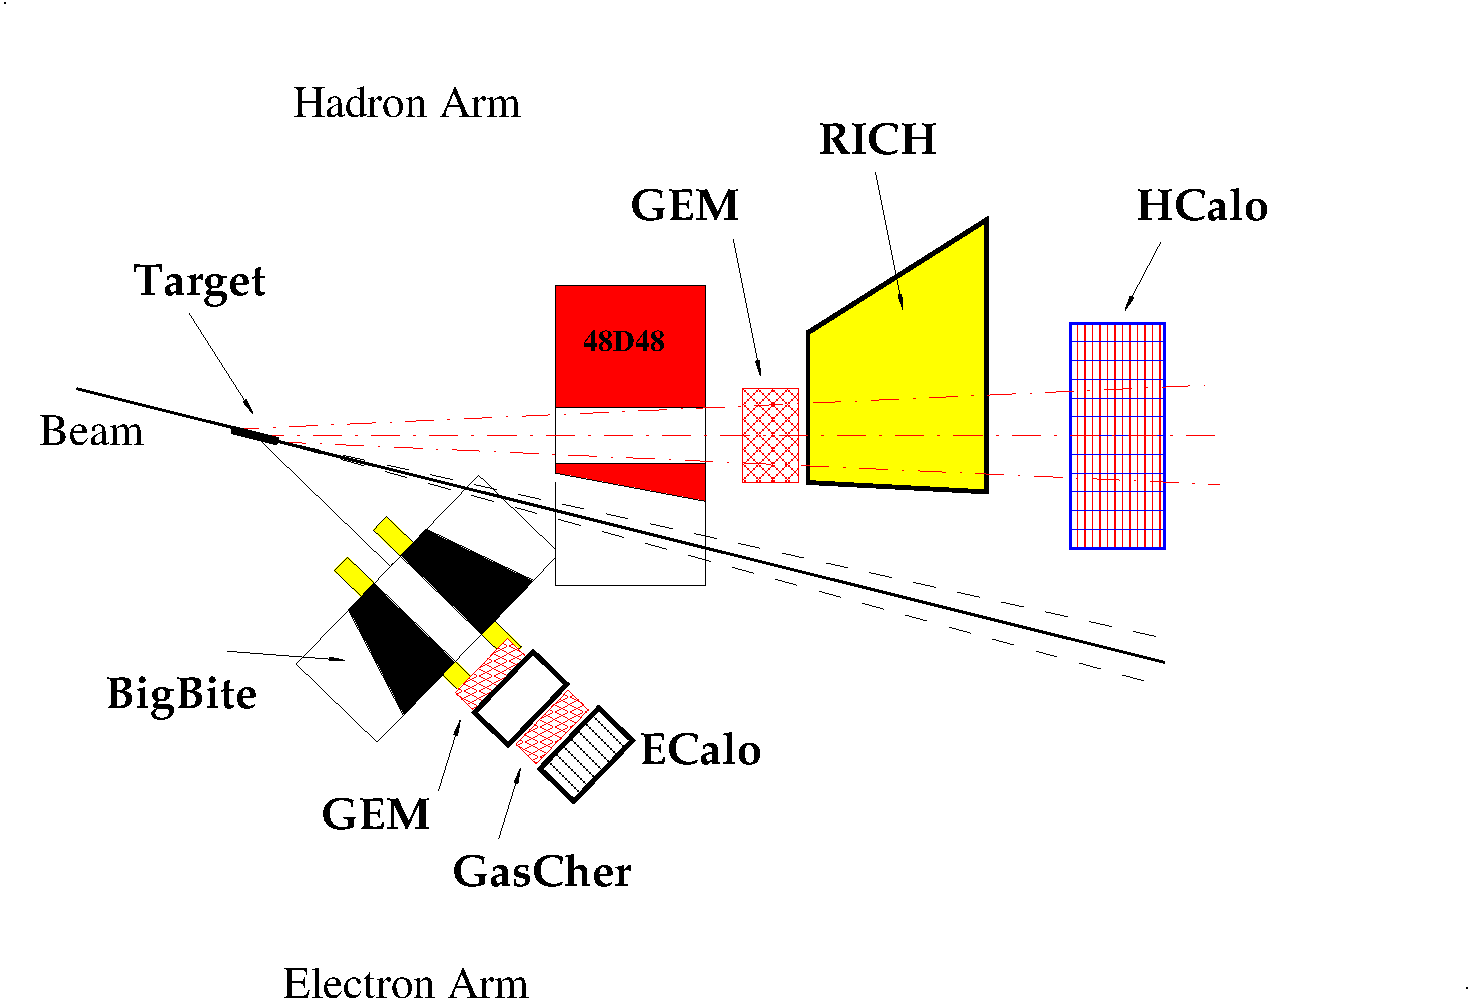
\includegraphics[width=.75\textwidth]{figures/SIDIS_layout.pdf}
  \end{center}
  \caption{\label{fig:cartoon} Schematic layout of the proposed measurements. The BigBite Spectrometer detects DIS electrons at a central angle of 30$^\circ$ on the beam right, while the Super BigBite Spectrometer detects SIDIS hadrons on the beam left in the vicinity of the momentum transfer direction at central angles of 14$^\circ$ and 10$^\circ$.}
\end{figure}
Figure~\ref{fig:cartoon} shows the basic layout of the experiment. BigBite will detect DIS electrons with momenta $p_e \ge 1$ GeV at a central angle of 30$^\circ$ on the beam right. Super BigBite (SBS) will detect SIDIS hadrons including $\pi^\pm$, $\pi^0$ and $K^\pm$ on the beam left, with data taking equally divided between central angles of 14$^\circ$ and 10$^\circ$. The trigger threshold of the SBS hadronic calorimeter (HCAL) will be set for the efficient detection of hadrons with momentum $P_h \ge 2$ GeV. 

The detector package of SBS will be oriented vertically behind the SBS magnet in the proposed experiment, leading to symmetric acceptances for positive and negative charged hadrons that are identical in first approximation. Moreover, the polarity of the SBS magnetic field will be periodically reversed, such that approximately half the data will be collected in up-bending and down-bending configurations for both positive and negative hadrons; the SBS polarity reversals will cancel the effects of any residual differences in acceptance/efficiency between positive and negative hadrons, which will drastically reduce the systematic uncertainties in the charge-sum and charge-difference asymmetries. Reversing the SBS magnet polarity also increases the $\phi_h$ acceptance by roughly $14\%$, and the $\phi_h$ acceptance of the combination of upbending and downbending configurations is also symmetric about $\phi_h = 0$. 
\subsection{High-Luminosity Polarized $^3$He Target}
\paragraph{}
The operation of polarized $^3$He targets at substantially higher luminosities than in previous experiments has been made possible by the recent development of targets using convection to more rapidly recirculate the $^3$He gas from the optical pumping chamber in which it is polarized to the target cell in which it is exposed to the beam~\cite{Helium3_target}. The $^3$He target in the proposed experiment has the same basic operating parameters as the target to be used in E12-09-018~\cite{SBS_SIDIS} and another approved SBS experiment E12-09-016~\cite{GEN2} that will measure the neutron electromagnetic form factor ratio $G_E^n/G_M^n$ up to $Q^2 \sim 10$ GeV$^2$. The target will be 60 cm thick along the beam direction at a pressure of 10.5 atm. The use of thin metal end windows to reduce backgrounds will allow an increase in the useful luminosity by a factor of 3-4 while only increasing the total luminosity by roughly a factor of 2 compared to representative experiments from the 6 GeV era, such as the E06-010 experiment~\cite{E06010_AUT_PRL}. The target in the proposed experiment differs from the other two SBS $^3$He experiments only in the orientation of the target polarization, which will be along the beam direction in this experiment. An in-beam $^3$He  polarization of 65\% is assumed throughout this proposal in the calculation of projected asymmetry uncertainties. 
\subsection{BigBite Spectrometer}
\paragraph{}
BigBite is a non-focusing magnetic spectrometer consisting of a vertical-bend dipole magnet with a maximum field-integral of approximately 1.0 T$\cdot$m that can be instrumented with a flexible configuration of detectors. At its maximum field setting, the BigBite dipole bends the trajectory of a $1.5$ GeV particle of charge $e$ by approximately 10 degrees, providing for moderate momentum resolution of approximately $1\%$ for charged-particle momenta up to several GeV. The BigBite spectrometer was first used at the NIKHEF facility~\cite{BigBite1998,BigBiteOptics1998} and was later installed in Hall A at Jefferson Lab, where it has been successfully used in several different experiments, including but not limited to the measurement of the neutron electric form factor $G_E^n$ up to $Q^2 = 3.4$ GeV$^2$~\cite{GEN2010}, SIDIS on a transversely polarized $^3$He target~\cite{E06010_AUT_PRL} and many other experiments that have completed data taking but are not yet published. In the $G_E^n$ and SIDIS experiments, BigBite was used as the electron spectrometer in coincidence with a hadron detector on the opposite side of the beamline. Following the 12 GeV upgrade, BigBite will be used in this role again in several approved experiments, including E12-09-016~\cite{GEN2} and E12-09-018~\cite{SBS_SIDIS}.

In order to tolerate the higher luminosities of planned experiments at 11 GeV, and to realize the improvements in tracking resolution needed to preserve the $\sim1\%$ momentum resolution of BigBite for higher-momentum particles at the same field integral, the BigBite drift chambers will be replaced with Gas Electron Multiplier (GEM) trackers~\cite{Sauli_GEM, GEM_test_1999}, which have been shown to have stable gain at charged-particle rates of up to 1 MHz/mm$^2$. A large number of GEM chambers are currently being produced at UVA and INFN for E12-07-109~\cite{GEP5}, a measurement of the proton electromagnetic form factor ratio $G_E^p/G_M^p$ to $Q^2 = 12$ GeV$^2$. The GEMs are modular in design, with an active area of up to 50 $\times$ 60 cm$^2$, and will be available to other experiments in Hall A when E12-07-109, which does not use BigBite, is not running. Another planned upgrade to the BigBite detector package for experiments at 11 GeV is a highly-segmented gas Cherenkov detector currently under construction at the College of William and Mary, which will improve electron identification in BigBite compared to 6 GeV experiments that primarily used the lead-glass calorimeter for this purpose.
\subsection{Super BigBite Spectrometer}
\paragraph{}
The Super BigBite Spectrometer (SBS)~\cite{SBS_CDR,SBS_CDR_NEW} is a device conceptually similar to BigBite. The SBS will use a ``48D48'' magnet acquired by JLab from BNL as a magnetic spectrometer, operated at a field integral of roughly 1.8 T$\cdot$m. The SBS will be capable of reaching forward scattering angles by means of a cut in the magnet yoke for passage of the beam pipe. In E12-07-109, which proposed to run at luminosities approaching $10^{39}$ cm$^{-2}$s$^{-1}$, the SBS will be instrumented with a proton polarimeter constructed from GEM trackers and CH$_2$ analyzers, and a hadronic calorimeter for triggering on high-momentum protons. % A large-acceptance proton polarimeter is required to extend the measurement of $G_E^p$ to large $Q^2$ because of the rapid decrease of the elastic scattering cross section. 
A significant challenge in the use of open-geometry spectrometers such as BigBite and SBS is the implementation of a trigger that is selective enough to reduce the data acquisition (DAQ) rate to a manageable level while maintaining high efficiency for the events of interest. The BigBite and SBS designs achieve this by exploiting the exponential decrease of the trigger rate as a function of the energy threshold in total-absorption calorimeters. Manageable trigger rates are achieved using a calorimeter-based coincidence trigger between two independent spectrometer arms, each with as high a threshold as the experiment physics goals and detector performance will allow. % This is in stark contrast to the small-acceptance, focusing magnetic spectrometers in Hall A\cite{HallANIM} and Hall C\cite{HornLongPaper}, in which particles are transported over much longer path lengths through evacuated magnetic field volumes into shielded detector enclosures with much lower background counting rates. In such a low-background environment, the trigger is usually based on the fast signals from thin plastic scintillators in order to maintain high trigger efficiency and minimal trigger bias. In an open-geometry configuration in which the detectors are in direct view of the target at a distance of less than ten meters, the background rates are high enough that this approach is no longer feasible. Instead,

All of the SBS experiments will make use of a hadronic calorimeter currently under construction at Carnegie Mellon University. The design of the calorimeter is very similar to that of the ``HCAL1'' detector used by the COMPASS experiment~\cite{HCAL1}, but with several improvements needed to meet the performance specifications of the SBS experiments. The calorimeter consists of a 12$\times$24 array of modules, each consisting of a stack of 40 alternating layers of 20 mm-thick iron and 5 mm-thick scintillator, with a frontal area of 15 $\times$ 15 cm$^2$. The design goals for HCAL include a high ($\gtrsim$ 95\%) trigger efficiency for protons with momenta from roughly 3-8 GeV at a threshold of 25\% of the average signal, a timing resolution of 1 ns or less, and a coordinate resolution better than 5 cm. To meet these requirements, the SBS HCAL will use fast scintillator and wavelength shifter materials and a novel light guide to collect the scintillation light onto two-inch-diameter PMTs with faster response time and higher quantum efficiency than those used by the COMPASS experiment. % The design of the HCAL for the SBS experiments has been the subject of an extensive simulation effort using the GEANT4 toolkit\cite{GEANT42003}.
In E12-09-018, the SBS HCAL will be used as a charged hadron trigger and will also detect $\pi^0$s. A Monte Carlo evaluation of the $\pi^0$ acceptance and reconstruction efficiency in the SBS showed that the $\pi^0$ statistics will be similar to those of charged kaons.

Two different types of GEM trackers are being constructed for the SBS experiments. The SBS front tracker GEMs, currently under construction at INFN, consist of six tracker planes, each consisting of three 40$\times$50 cm$^2$ GEM modules, arranged vertically for a total area per plane of 40$\times$150 cm$^2$. In the $G_E^p$ experiment, the front tracker is used to measure the kinematics of the scattered proton in elastic $ep$ scattering and to define the incident proton trajectory before the polarization-analyzing scattering in CH$_2$. The front tracker GEMs are subject to the most stringent performance requirements because they are in direct view of the target at a luminosity of $\sim 8\times 10^{38}$ cm$^{-2}$ s$^{-1}$, and experience soft-photon-induced background hit rates of roughly 400 kHz/cm$^2$~\cite{SBS_CDR_NEW}. To realize efficient track reconstruction capability with low false-positives in this environment, a spatial resolution of 70 $\mu$m is required. To realize this spatial resolution, a readout strip pitch of 0.4 mm in both directions is used, leading to a total of about 60,000 readout channels for the entire front tracker. 

The SBS polarimeter GEMs, currently under construction at UVA, are subject to different and less stringent performance requirements. These GEMs are used to track protons scattered in CH$_2$ analyzers. They are shielded from the target by the CH$_2$ analyzers and therefore have lower background rates than the front trackers. Only moderate spatial resolution is required for reliable tracking and sufficient resolution of the proton scattering angles in the CH$_2$ analyzers. Although the readout planes for the polarimeter GEMs have the same 0.4 mm strip pitch as the front tracker GEMs, the less demanding resolution requirement and the lower expected occupancy allow for two readout strips to be combined into a single readout channel to reduce the number of electronics channels required. On the other hand, a larger area is needed for the polarimeter GEMs in order to provide complete azimuthal acceptance for protons scattered by up to 10 degrees in the CH$_2$. A total of 40 GEM modules of area 50$\times$60 cm$^2$ will be produced. These modules will be arranged into two trackers, each consisting of five planes of area 60 $\times$ 200 cm$^2$. The first polarimeter tracker will be located between the two CH$_2$ analyzers, while the second will be located between the second CH$_2$ analyzer and HCAL. %The use of two polarimeters in series, each approximately one nuclear interaction length thick, has been shown to lead to a $\sim50\%$ efficiency gain relative to a single polarimeter of equivalent thickness~\cite{GEP3,Ay_pCH2}. 
In E12-09-018 and in the proposed experiment, GEM-based trackers for BigBite and SBS will be assembled from a combination of the front tracker and polarimeter GEM modules. Because the total luminosity in E12-09-018 is a factor of 40 lower than E12-07-109, the background environment in SBS is much more forgiving, such that a large-area tracker assembled from polarimeter GEM modules will have sufficient tracking performance and resolution.

\subsection{Ring-Imaging Cherenkov detector for SBS}
%\subsubsection{RICH Overview}
The designs of SBS and BigBite lend themselves naturally to the study of SIDIS at high $x$ and $Q^2$. To make the SBS a viable hadron spectrometer for SIDIS requires a robust particle identification (PID) capability. The dual-radiator Ring-Imaging Cherenkov (RICH) detector from the HERMES experiment~\cite{HERMES_RICH_long_NIM}, which became available following the end of the HERMES experiment, was quickly recognized as an excellent low-cost solution for PID in the SBS. The HERMES RICH detector uses aerogel with a refractive index $n = 1.0304$ and C$_4$F$_{10}$ gas with $n = 1.00137$ to provide redundant separation of pions, kaons and protons for momenta ranging from the kaon aerogel Cherenkov threshold of 2 GeV up to a limit of 15 GeV determined by the resolution of the reconstructed emission angle in the gas radiator. Cherenkov photons emitted by above-threshold charged hadrons in the aerogel and gas radiators are collected by a large-area spherical mirror with a radius of curvature of 2.2 m onto an array of 1,934 3/4''-diameter photomultiplier tubes (PMTs). The HERMES RICH consists of two identical detector halves on opposite sides of the HERA beam pipe in the HERMES spectrometer. One of the detector halves has been preserved and transferred to JLab for use in SBS, as well as the aerogel wall from the second half.
\begin{figure}[h]
  \begin{center}
    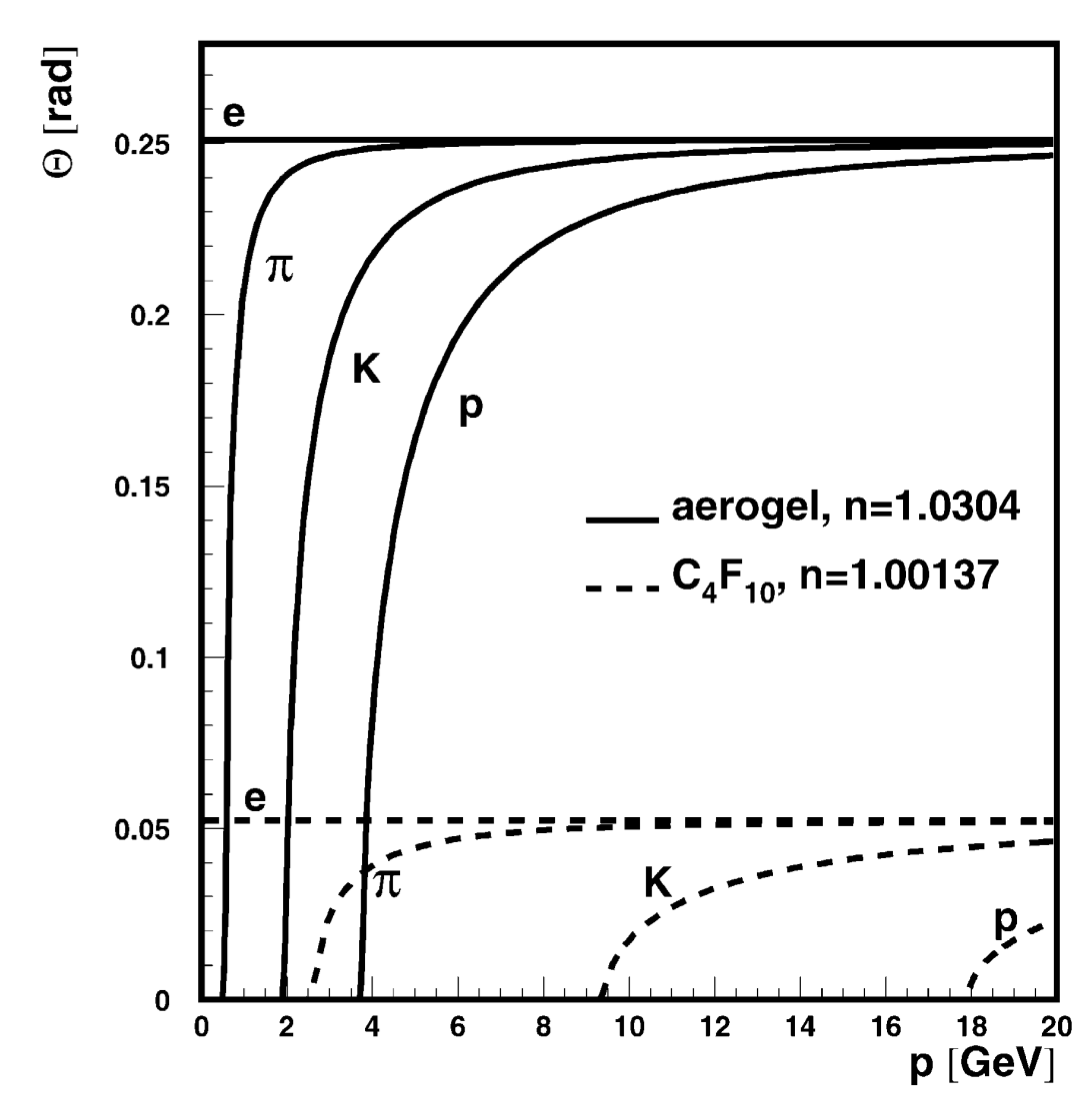
\includegraphics[width=0.33\textwidth]{figures/thetaC_vs_p.png}
    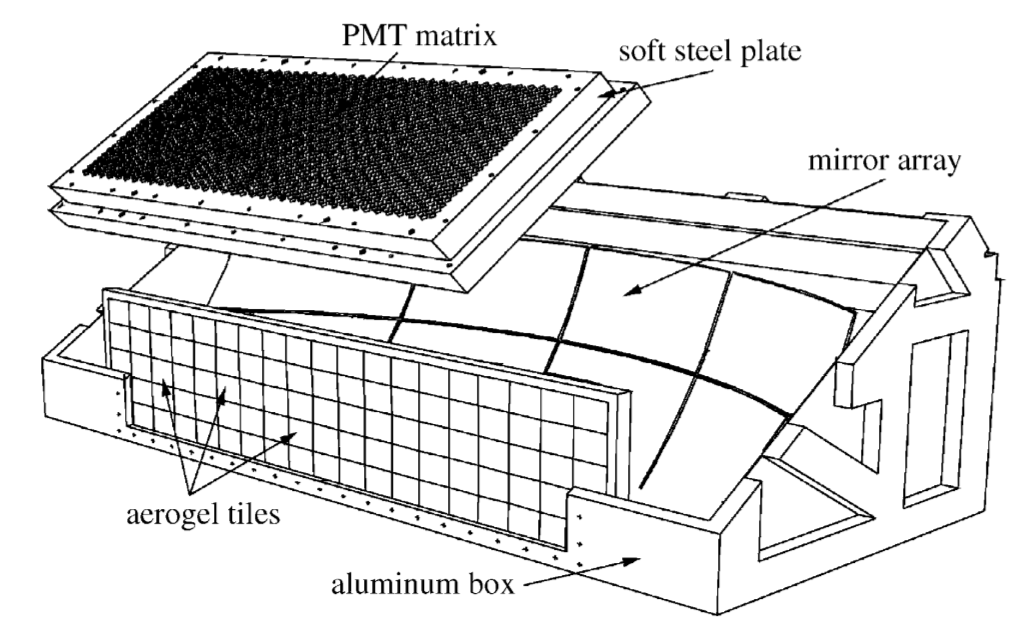
\includegraphics[width=0.5\textwidth]{figures/RICH_schematic.png}
  \end{center}
  \caption{\label{RICHfig1} Left: Cherenkov emission angle $\theta$ as a function of particle momentum $p$ for the dual-radiator HERMES RICH counter. Right: layout of the major components of the RICH. Figures reproduced from~\cite{HERMES_RICH_long_NIM}.}
\end{figure}
Fig.~\ref{RICHfig1} shows the basic design and working principle of the RICH. The aerogel wall consists of an array of 5 rows $\times$ 17 columns of aerogel tiles stacked 5 tiles deep. The average tile dimensions are (11.4 $\times$ 11.4 $\times$ 1.13) cm$^3$. % The entry and exit windows consist of 1 mm-thick aluminum. The dimensions of the RICH entry (exit) window are 187.7 $\times$ 46.4 cm$^2$ (257.0 $\times$ 59.0 cm$^2$). 

%\subsubsection{Simulations of the HERMES RICH in SBS/E12-09-018}
Detailed Monte Carlo simulations of the HERMES RICH in SBS were carried out to determine the background rates in the PMTs and the useful acceptance of the RICH; i.e., the range of particle trajectories for which adequate PID performance is expected.
\begin{figure}[h]
  \begin{center}
    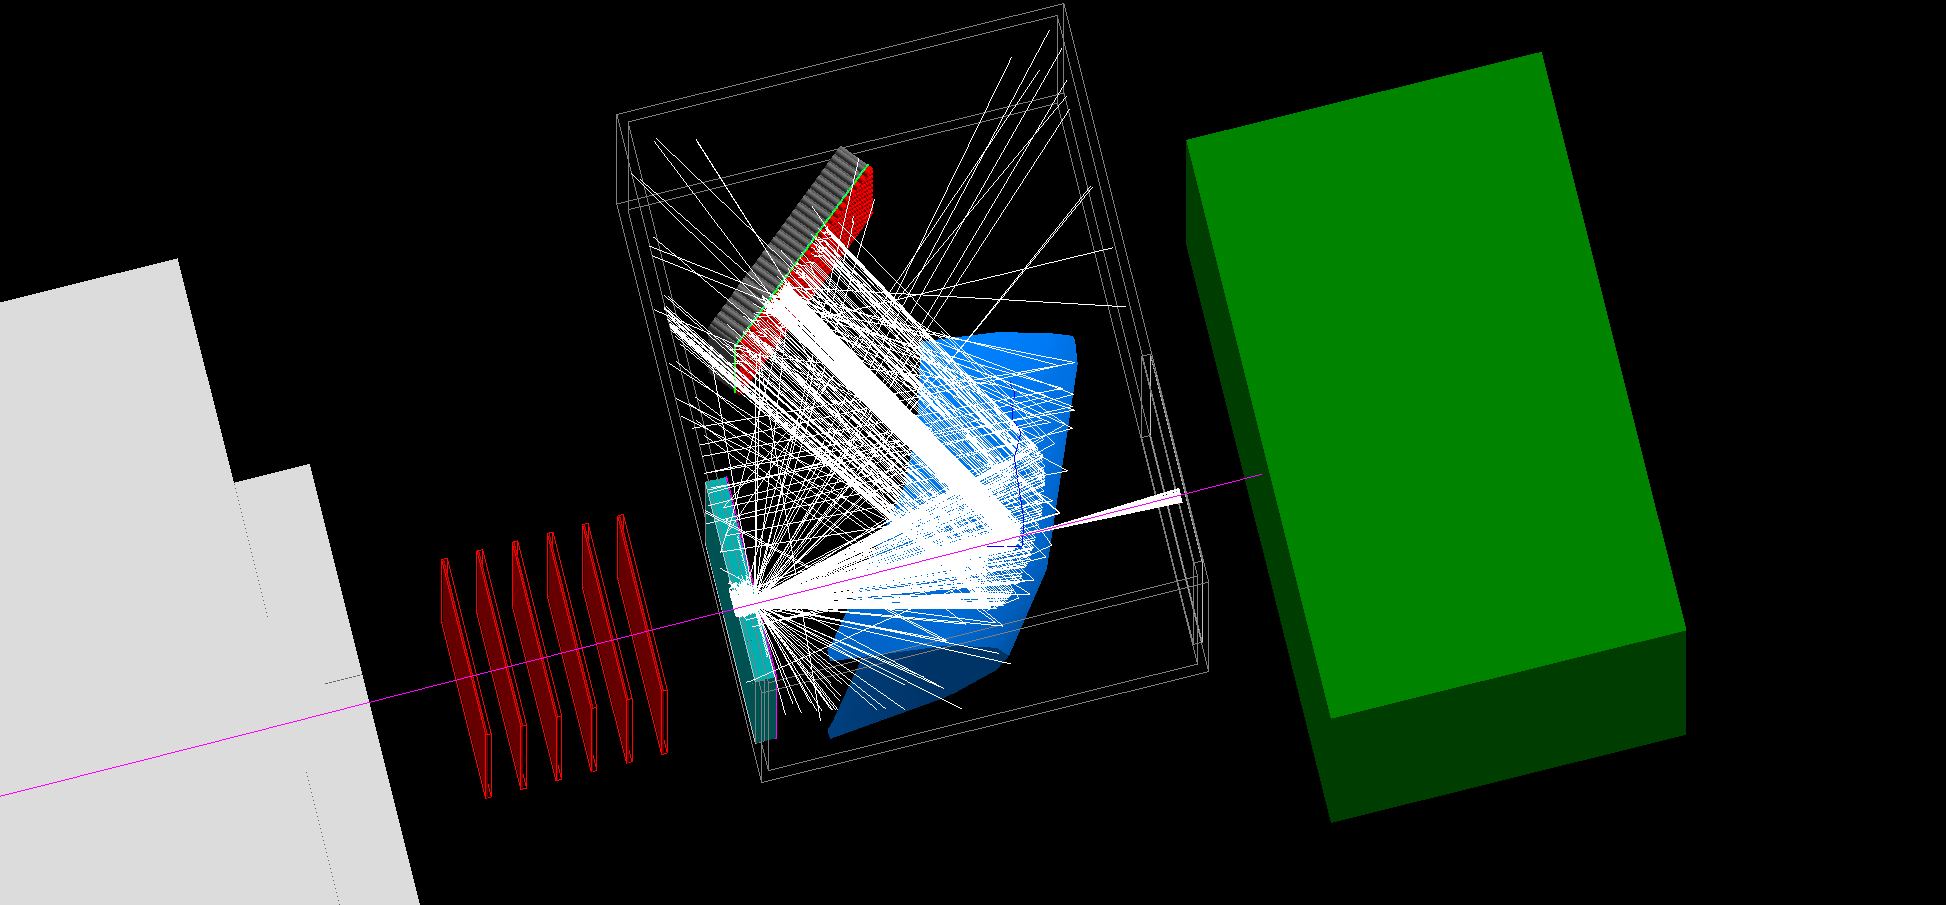
\includegraphics[width=.48\textwidth]{figures/RICH_5GEV_pion.png}
    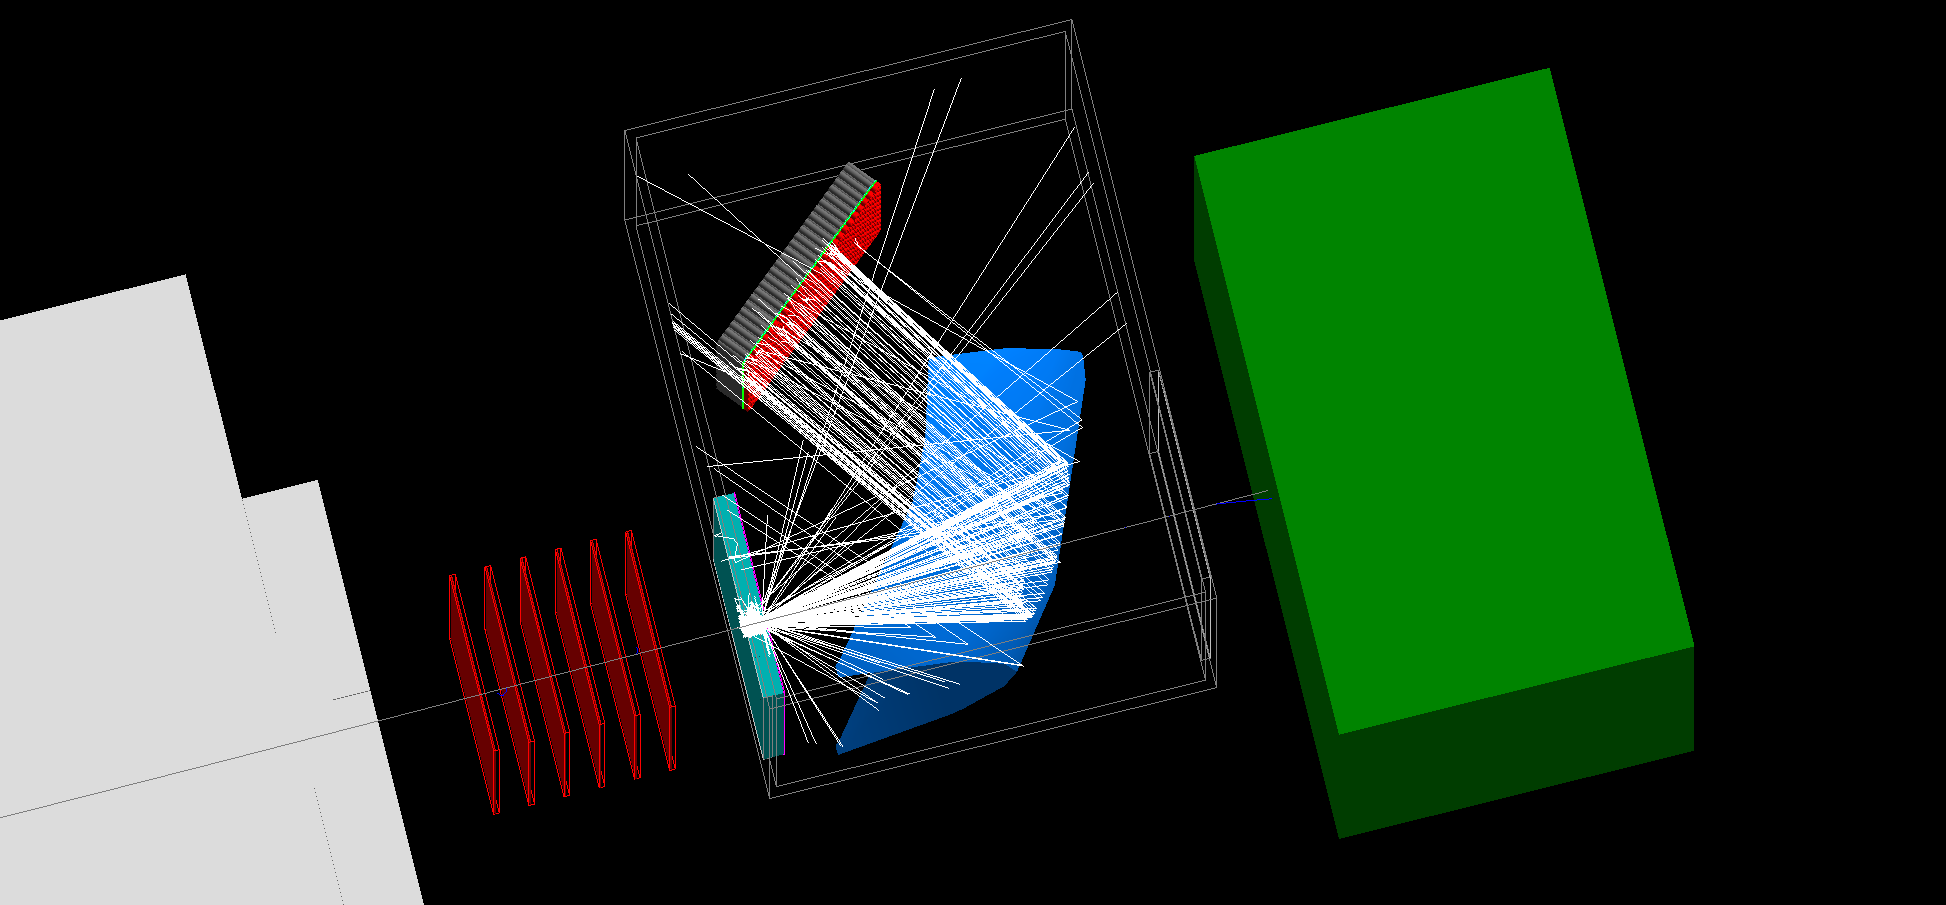
\includegraphics[width=.48\textwidth]{figures/RICH_5GEV_kaon.png}
  \end{center}
  \caption{\label{RICHG4} Layout of the HERMES RICH in the Monte Carlo simulation of E12-09-018. Left: A pion with a momentum of 5 GeV emits Cherenkov radiation in aerogel and gas. Right: A kaon moving along the same trajectory at the same momentum only produces Cherenkov light in aerogel at smaller emission angles. The spherical mirror collects the light onto the PMT matrix. }
\end{figure}
Fig.~\ref{RICHG4} shows the layout of the RICH in the SBS Monte Carlo simulation using the GEANT4 toolkit~\cite{GEANT42003}, and examples of the Cherenkov light emitted by a pion and a kaon with identical trajectories. The simulation includes details of BigBite, the SBS magnet, the $^3$He target, the GEM tracker, the RICH, HCAL, and the materials along the beamline. Preliminary background rate calculations for the PAC38 proposal for E12-09-018~\cite{SBS_SIDIS} indicated an average PMT occupancy\footnote{``Occupancy'' is defined as the probability of an accidental background hit within the timing window of an event.} of 0.1\%, assuming the RICH PMT signals can be correlated in time with the signals from the other detectors to within $\pm$5 ns. Such an occupancy leads to very high signal/noise ratios for the PID analysis. To achieve such a small effective timing window requires the implementation of a TDC readout for the RICH PMTs in SBS, a feature which was absent from the HERMES setup because the beam repetition rate at HERA was such that the smallest useful time window for detector readout was 100 ns.

\begin{figure}[h]
  \begin{center}
    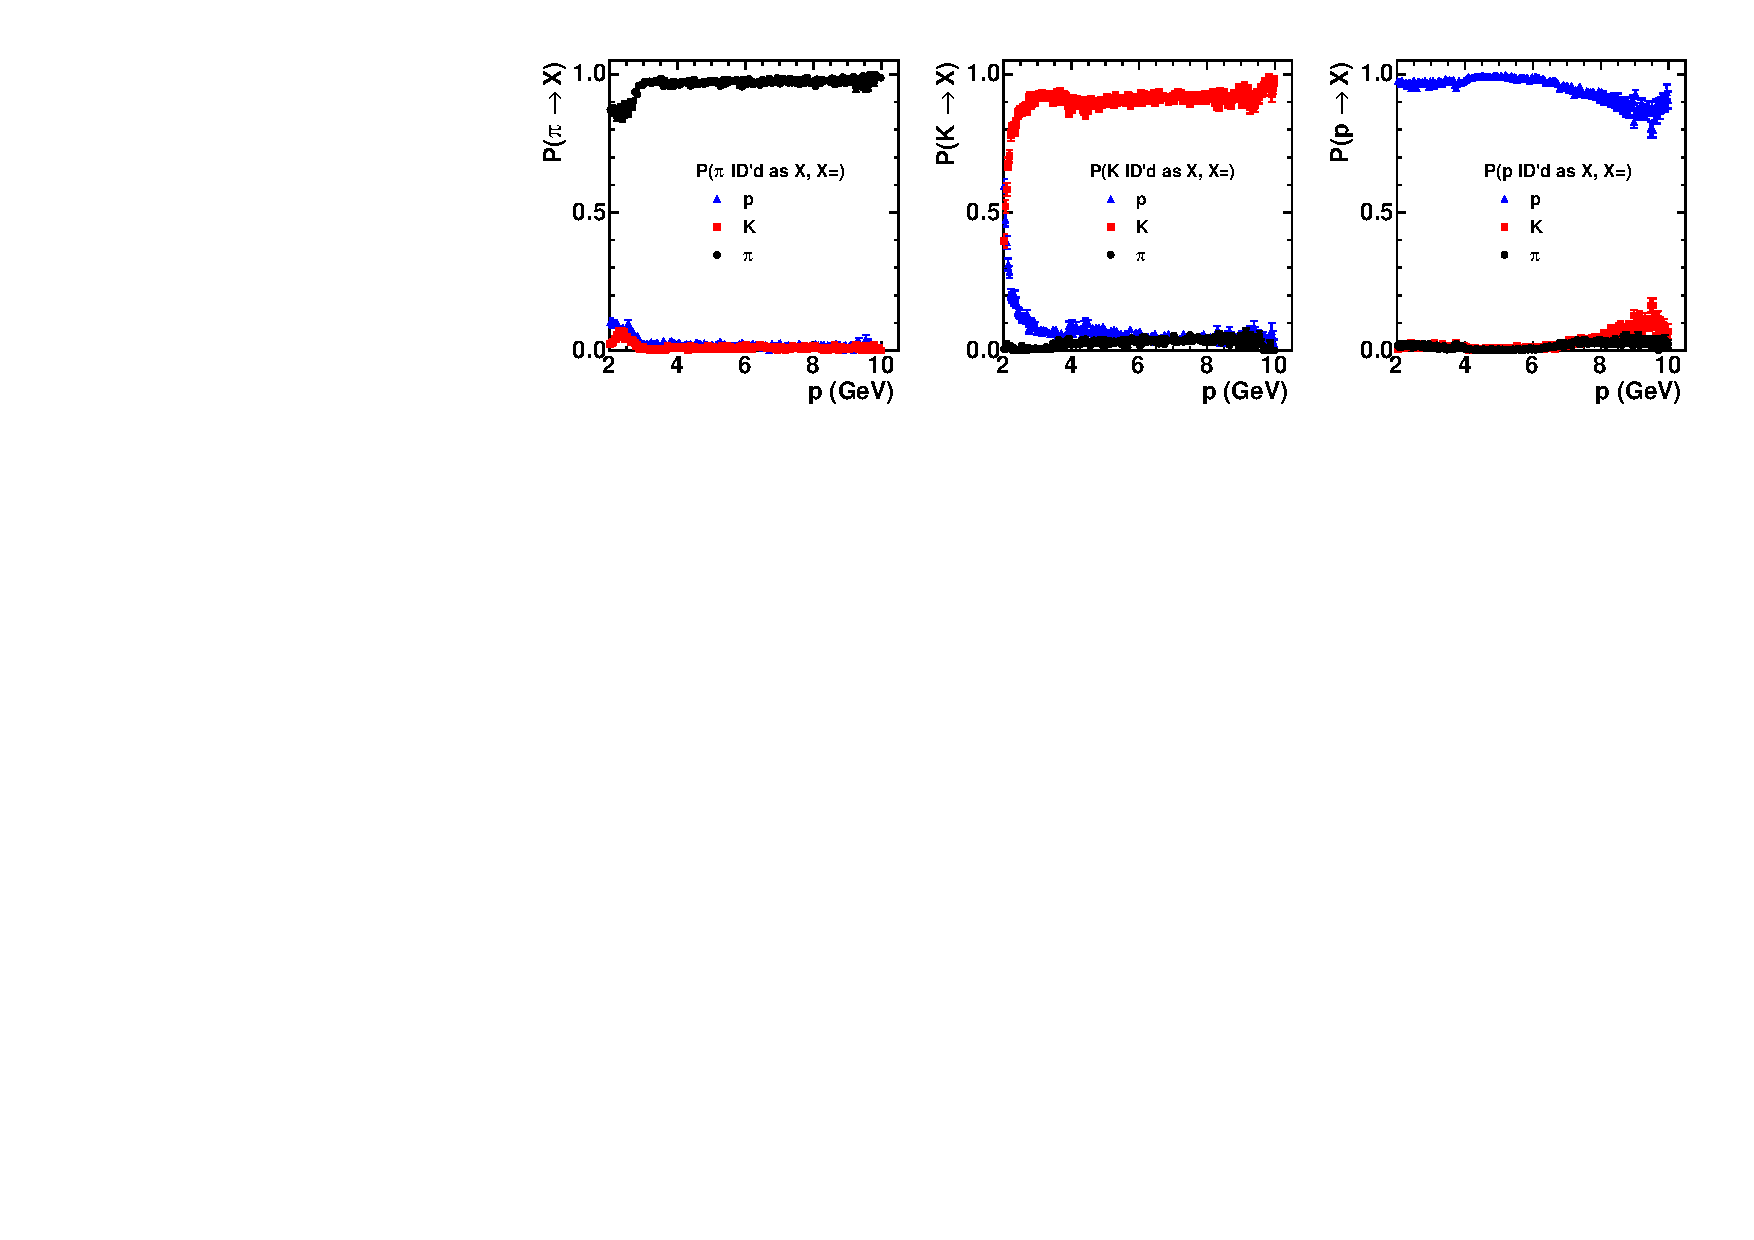
\includegraphics[width=0.98\textwidth]{figures/SBS_PIDfig.pdf}
  \end{center}
  \caption{\label{RICHfig2} PID results from SBS Monte Carlo simulation. Particle ID probabilities as a function of momentum for pions (left), kaons (center) and protons (right). Results are preliminary and can be improved via further optimization of the PID algorithm.}
\end{figure}
Fig.~\ref{RICHfig2} shows preliminary PID results from the SBS RICH Monte Carlo simulation. The PID performance is characterized by the probability $P_{ij}$ of assigning particle hypothesis $j$ to a track with known true particle type $i$ and reconstructed\footnote{The momentum resolution of SBS is $\sigma_p/p \approx 1\%$.} momentum $p$. The PID assignment is made based on a simplified version of the inverse ray tracing algorithm described in~\cite{HERMES_RICH_long_NIM}. The only requirement imposed on the selection of MC events for the PID analysis is the presence of a track, so that the misidentification probabilities shown include the effects of acceptance mismatch (i.e., those events which have small or non-existent signals because of a failure to produce and/or collect sufficient Cherenkov light). These preliminary results already demonstrate that the efficiency and purity of the PID analysis are high across the entire momentum range of interest, and that the geometry of the RICH does not significantly reduce the SBS acceptance relative to the combined acceptance of the SBS magnet and GEM tracker. Of particular importance is the low ($\lesssim 1\%$) probability to misidentify pions as kaons above the pion gas threshold of $\sim$2.7 GeV, since the expected flux of pions is about ten times that of kaons in E12-09-018.

\section{Experiment Plan and Expected Results}
\subsection{Monte Carlo Simulation}
\begin{figure}[h]
  \begin{center}
    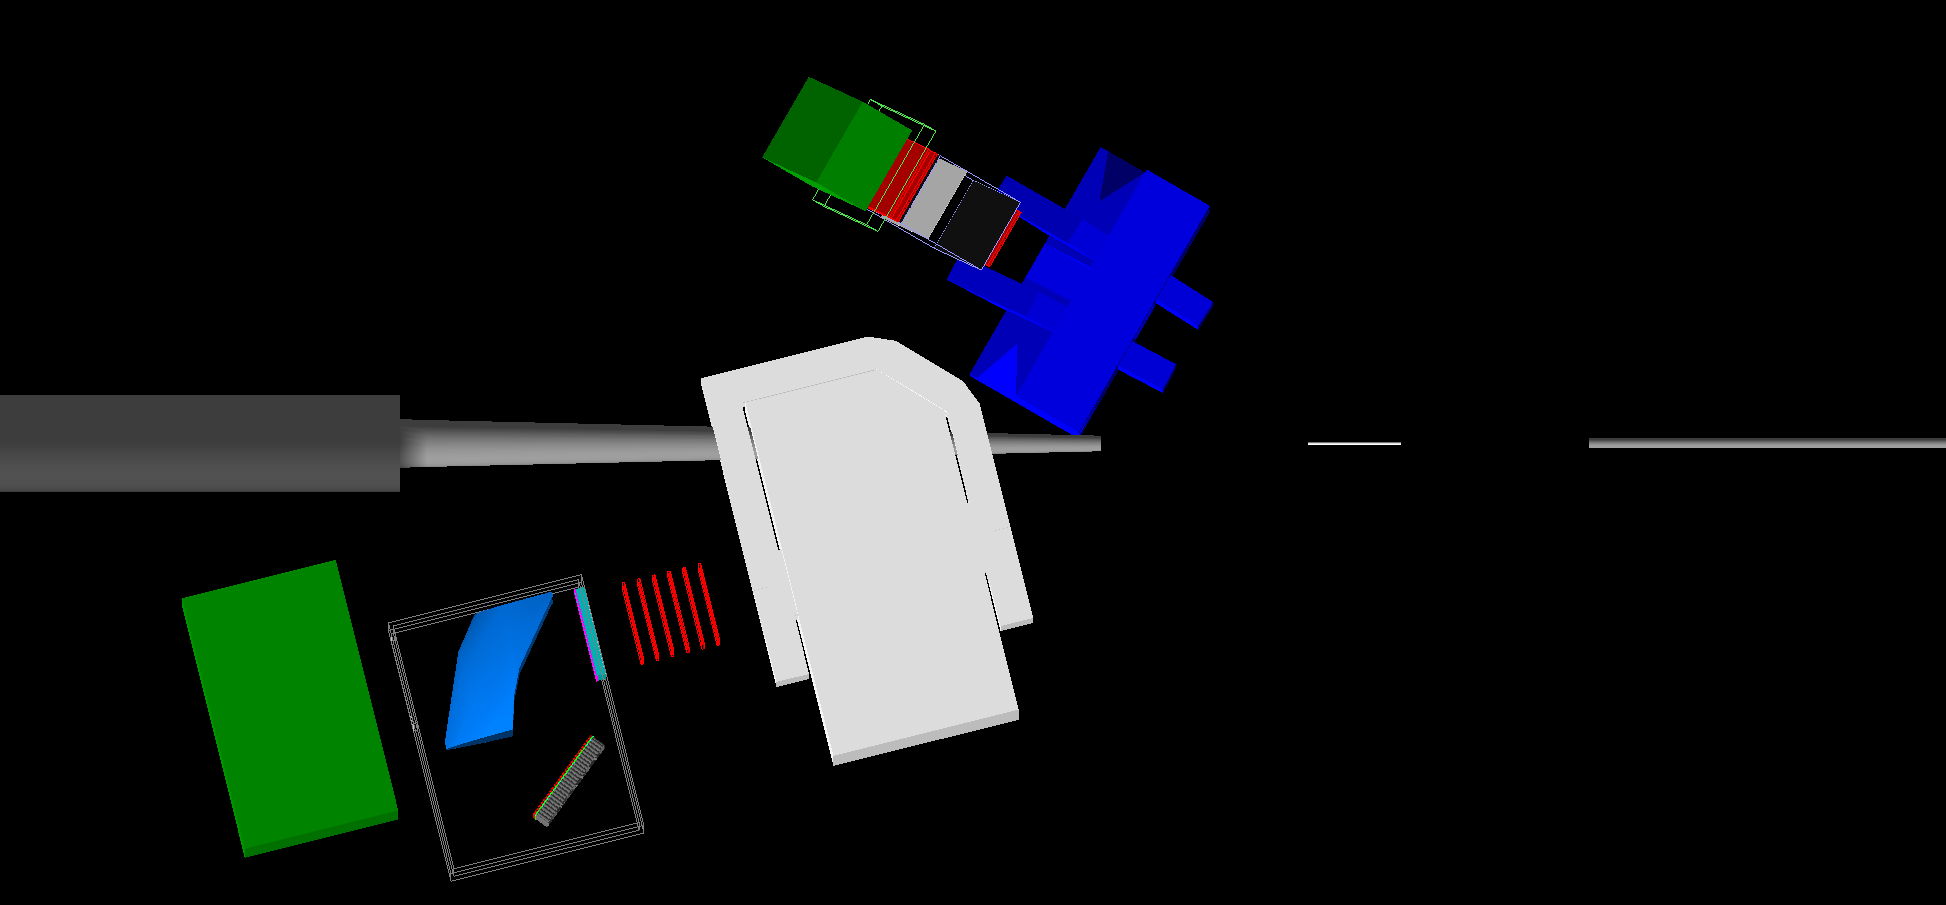
\includegraphics[width=.48\textwidth]{figures/SIDISlayout14deg.png}
    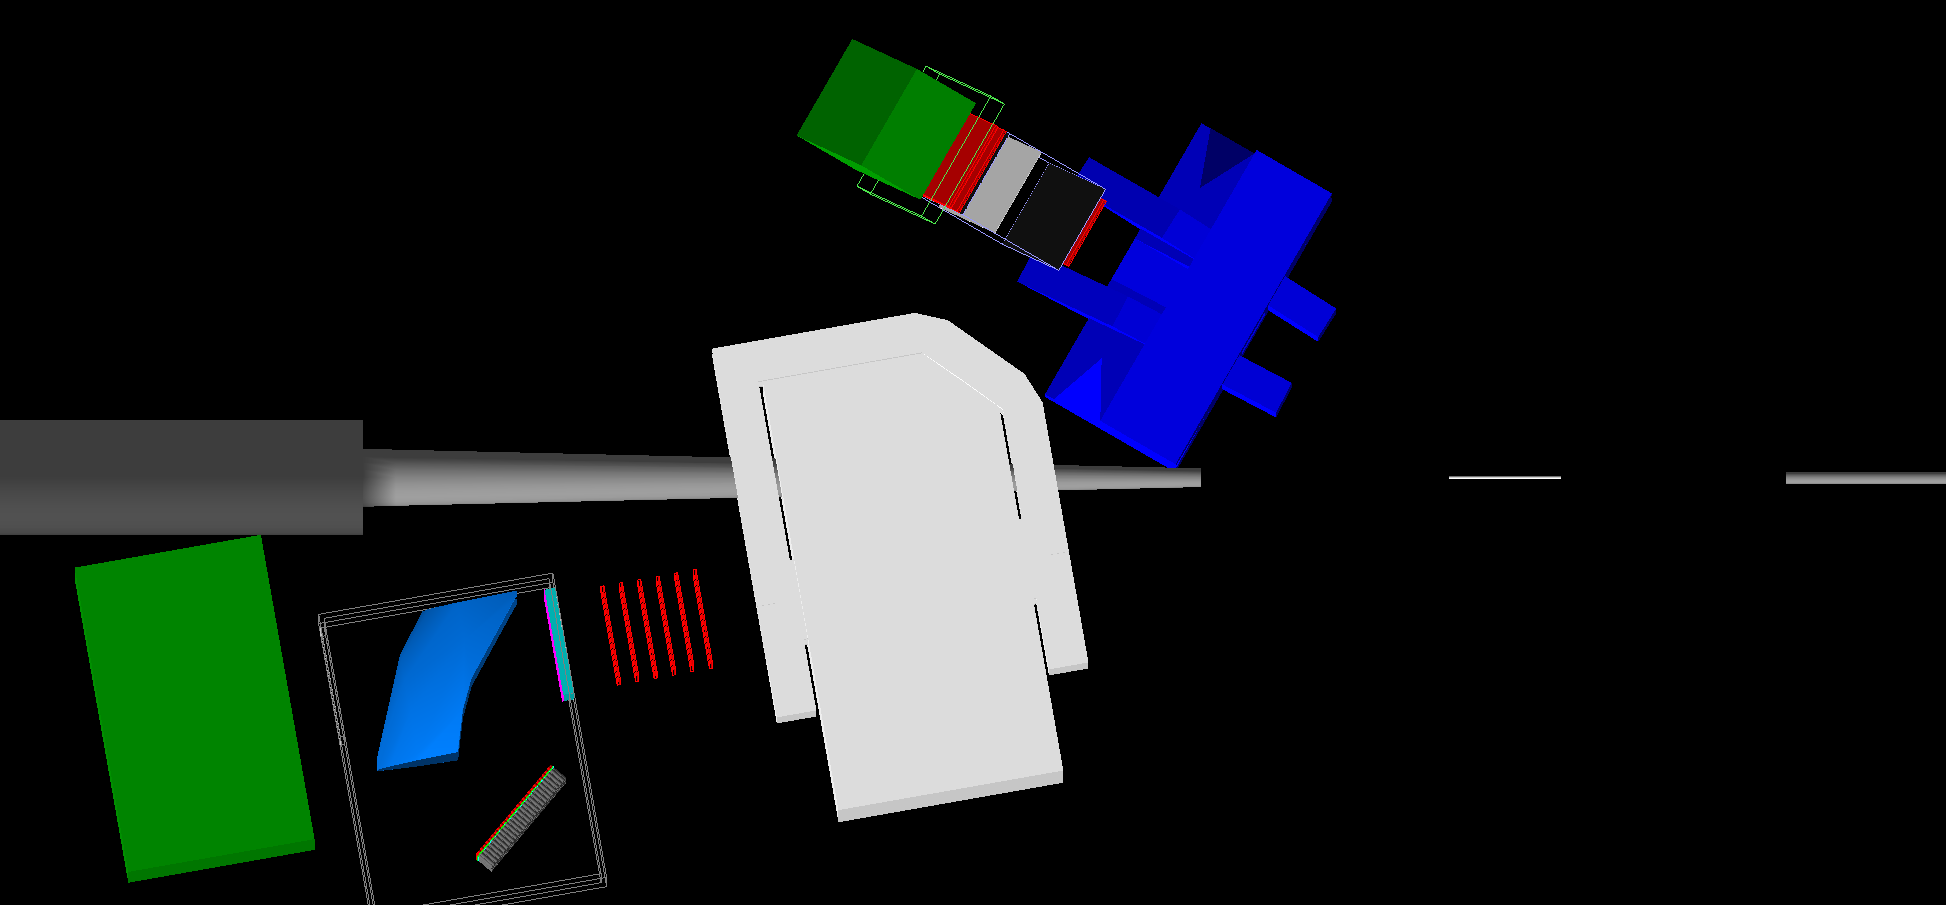
\includegraphics[width=.48\textwidth]{figures/SIDISlayout10deg.png}
  \end{center}
  \caption{\label{fig:layout} GEANT4 Monte Carlo model of the proposed experiment. Left: with SBS at a central angle of 14$^\circ$ at a distance of 2.5 meters, identical to approved experiment E12-09-018. Right: with SBS at a central angle of 10$^\circ$ at a distance of 2.6 meters.}
\end{figure}
\paragraph{}
Figure~\ref{fig:layout} shows the GEANT4 model of the proposed experiment in each of the two proposed SBS angle settings. The simulation includes the detailed geometries and field layouts of both magnets, the essential features of the $^3$He target and the Hall A beamline, and realistic models of the detectors, which include the GEM tracker, the RICH and the HCAL for the hadron arm, and a GEM-based tracker, gas Cherenkov counter and electromagnetic calorimeter for the electron arm. SIDIS events were generated separately for each hadron species and propagated through the GEANT4 model. For all events, a good electron track in BigBite and above-threshold energy deposition in the BigBite calorimeter were required. For charged hadrons, a good track in SBS and above-threshold energy deposition in HCAL were required. The preliminary Monte Carlo studies of the RICH PID performance in SBS (see Fig.~\ref{RICHfig2}) already show that the acceptance of the RICH does not significantly reduce the useful acceptance of SBS for high-performance PID, relative to the acceptance defined by the magnet gap and the tracker area. Therefore, because the GEANT4 simulation of Cherenkov radiation in the SBS RICH is computationally expensive, the RICH was not included in the analysis for rate estimates and asymmetry uncertainty projections.  For $\pi^0$ events, both $\pi^0$ decay photons were required in HCAL with a minimum separation of one pixel. The following global cuts were applied to the ``true'' (nucleon rest frame) kinematics of generated SIDIS events:
\begin{itemize}
\item $Q^2 \ge 1$ GeV$^2$: Standard DIS cut. 
\item $W \ge 2$ GeV: Standard DIS cut to avoid the nucleon resonance region.
\item $M_X \ge 1.5$ GeV: Large missing-mass cut to avoid the exclusive and resonance regions of $n(e,e'h)X$.
\item $P_h \ge 2$ GeV: Minimum hadron momentum to minimize effects of nuclear final-state-interactions and target fragmentation.
\item $y \le 0.9$: Maximum fractional electron energy loss to avoid large QED radiative corrections, as well as large pair-production backgrounds present at low electron energies.
\item $P_e \ge 1$ GeV: ``Trigger threshold'' for BigBite; redundant with $y$ cut. 
\end{itemize}
\subsection{SIDIS Cross Section Model}
\paragraph{} For the purpose of rate estimation for this proposal, the unpolarized SIDIS cross section was calculated using a naive, leading-order, leading-twist approximation with the CTEQ6 PDFs~\cite{CTEQ6} and the DSS2007 fragmentation functions~\cite{DSS2007} for pions and kaons, neglecting any $\phi_h$ dependence. The unpolarized differential scattering cross section is given in this simple model by 
\begin{eqnarray}
  \frac{d\sigma}{dE'_e d\Omega_e dz dp_T^2 d\phi_h} &=& \frac{4\alpha^2 {E'_e}^2}{Q^4}\left[\frac{2H_1}{M} \sin^2 \left(\frac{\theta_e}{2}\right) + \frac{H_2}{\nu} \cos^2\left(\frac{\theta_e}{2}\right)\right], \label{sidisxsec}
\end{eqnarray}
where $E'_e$ is the scattered electron energy, $M$ is the nucleon mass, $\theta_e$ is the electron scattering angle, $\nu$ is the electron energy loss in the target rest frame, and the SIDIS structure function $H_2$ is given at leading order by
\begin{eqnarray}
  H_2(x, Q^2, z, p_T^2) &=& x \sum_q e_q^2 q(x,Q^2) D^h_q(z,Q^2) \frac{b_q^h}{2\pi}e^{-b_q^h p_T^2}.
\end{eqnarray}
Six light quark flavors $q = u,d,s, \bar{u}, \bar{d}, \bar{s}$ are included in the sum. $q(x,Q^2)$ is the unpolarized PDF for quark flavor $q$ and $D_h^q(z,Q^2)$ is the unpolarized fragmentation function for quark $q$ to hadron $h$. A factorized Gaussian transverse momentum dependence is assumed, with a flavor-independent average width given by:
\begin{eqnarray}
  b_q^h &=& \frac{1}{z^2\left<k^2_\perp\right> + \left<p_\perp^2 \right>}, 
\end{eqnarray}
where $\left<k^2_\perp\right>$ is the transverse momentum width of the initial quark distribution and $ \left<p_\perp^2 \right>$ is the width of the transverse momentum distribution of hadrons produced in the fragmentation of the recoiling quark. For the purposes of rate estimates for this proposal, constant values $\left<k^2_\perp\right> = 0.25$ GeV$^2$ and  $ \left<p_\perp^2 \right> = 0.20$ GeV$^2$ were assumed, following Ref.~\cite{PhysRevD.71.074006}. The Callan-Gross relation $H_2 = 2xH_1$ is assumed for the SIDIS structure functions, implying neglect of the longitudinal virtual photoabsorbtion cross section. The kinematic coverages and rate estimates shown in the next sections correspond to the simplified SIDIS cross section model of Eqn.~\eqref{sidisxsec} convoluted with the combined acceptance of the two-spectrometer setup.

SIDIS events on $^3$He ``smeared'' by the Fermi motion of the initial nucleons were generated in the GEANT4 simulation using the following procedure. First, the nucleon participating in the scattering event is chosen randomly; i.e., a neutron (proton) is chosen with probability $\frac{1}{3}$ ($\frac{2}{3}$). After choosing the initial nucleon, its initial momentum is sampled from the neutron (proton) momentum distribution in $^3$He obtained from a fit to the results of a calculation using the Argonne V18 potential, and its initial direction of motion is chosen randomly. The polar ($\cos \theta_{e/h}$) and azimuthal ($\phi_{e/h}$) scattering angles and energies $E'_{e/h}$ of outgoing particles in the \emph{lab frame} are generated randomly within limits chosen to populate the full solid angle and momentum acceptance of both spectrometers. The initial and final electron and nucleon four-momenta are then boosted to the nucleon rest frame, and the SIDIS cross section is computed using Eqn.~\eqref{sidisxsec}. If the nucleon participating in the scattering is a neutron, the cross section is obtained from that on a proton by interchanging $u$ and $d$ quarks. The ``true'' (nucleon rest frame) SIDIS kinematics are also calculated. Finally, the lab-frame cross section is computed from the nucleon-rest-frame cross section by accounting for the modification of the flux factor by the boost due to the fact that the collision in the lab frame is no longer collinear\footnote{The flux factor $F \propto \left| \mathbf{v}_e - \mathbf{v}_N\right|$ is the only part of the cross section which is not Lorentz-invariant, but has the Lorentz transformation properties of a cross-sectional area.}. The weight of each event is then calculated by multiplying the lab frame differential cross section by the Lorentz-invariant phase space volume of event generation and the integrated luminosity and dividing by the number of generated events. The weight thus defined represents the expected number of experimental counts corresponding to each Monte Carlo event. By keeping track of the identity of the nucleon participating in the collision, the dilution factors relating the $^3$He asymmetry to the neutron asymmetry are also determined. 
\subsection{SIDIS Kinematic Coverage}
%\label{phasespaceplots}
% \begin{figure}[h]
%   \begin{center}
%     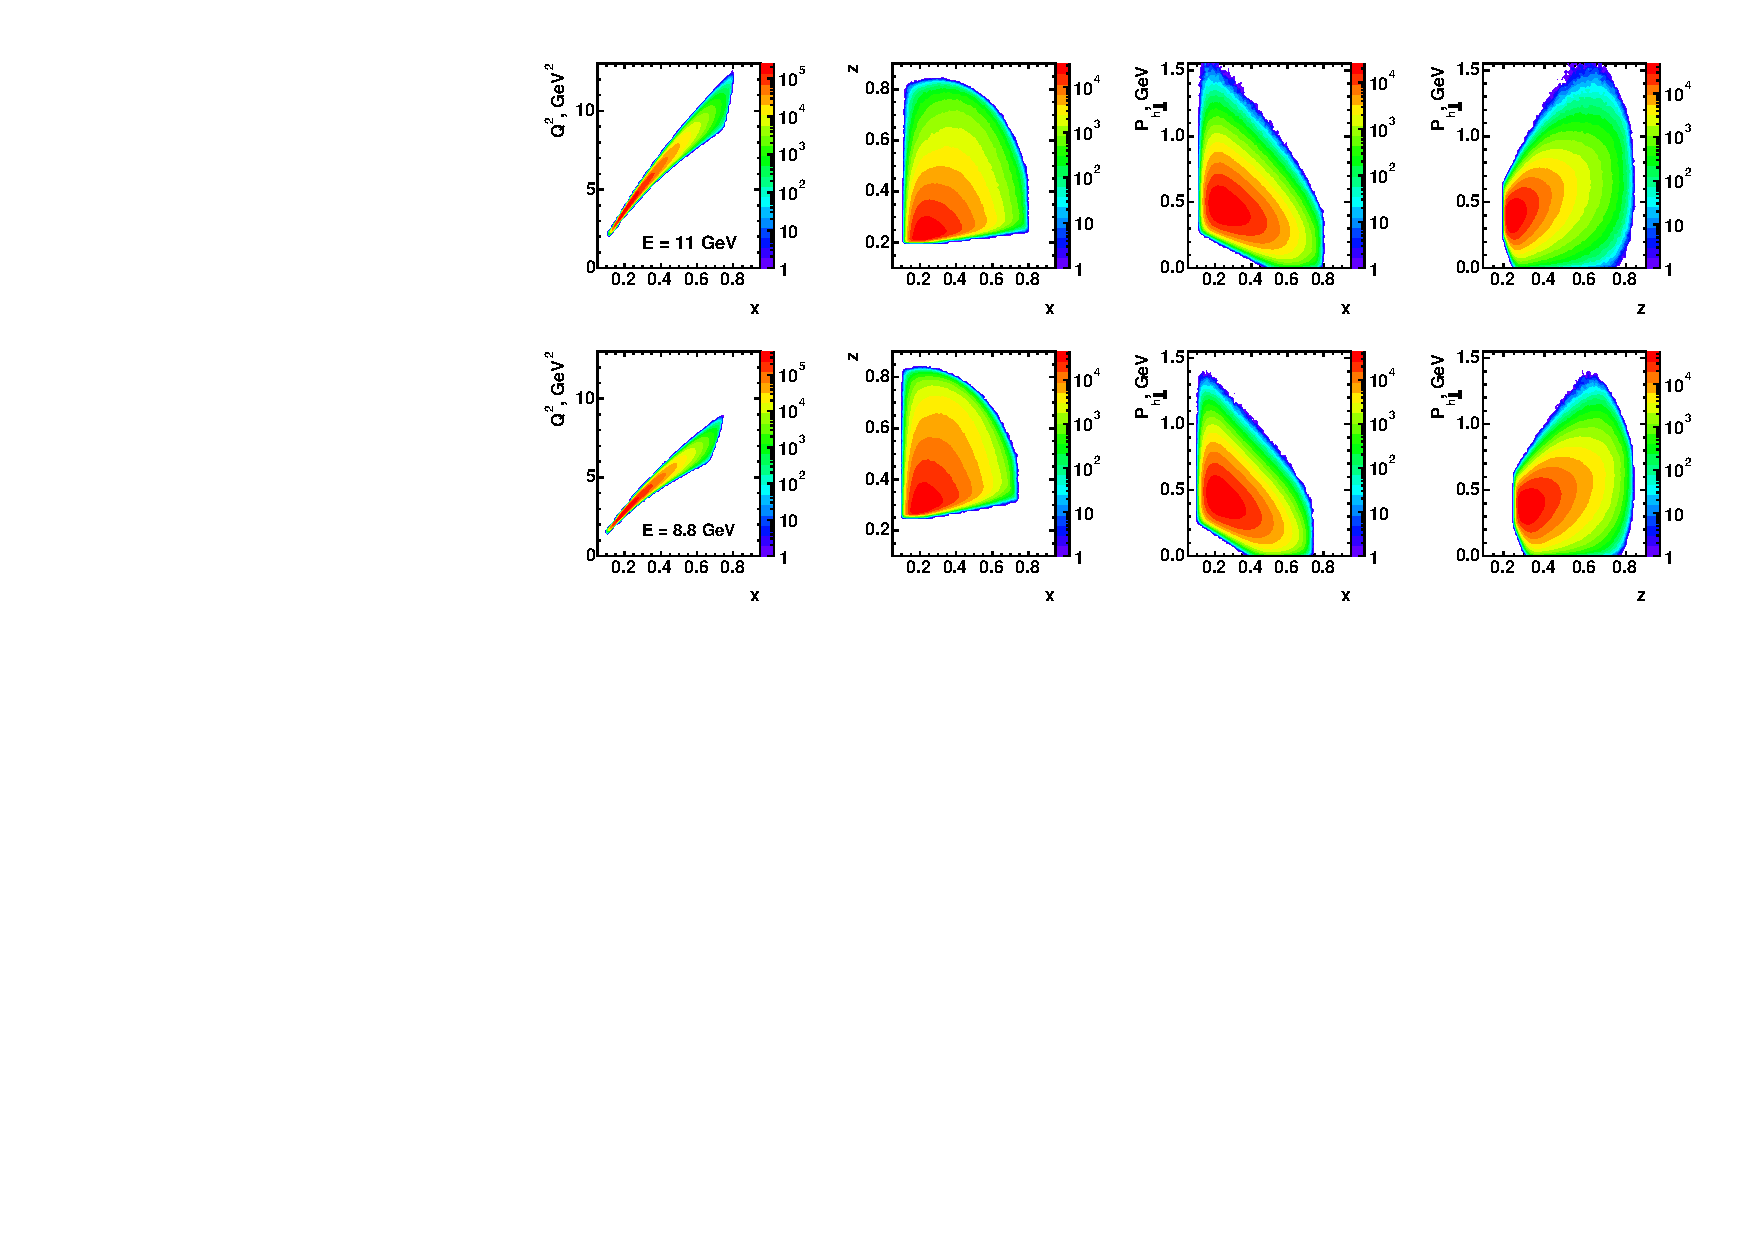
\includegraphics[width=.98\textwidth]{figures/phase_space.pdf}
%   \end{center}
%   \caption{\label{phasespace14deg} SIDIS kinematic coverage for the 14 degree setting at the two beam energies of 11 and 8.8 GeV.}
% \end{figure}
\paragraph{}
\begin{figure}[h]
  \begin{center}
    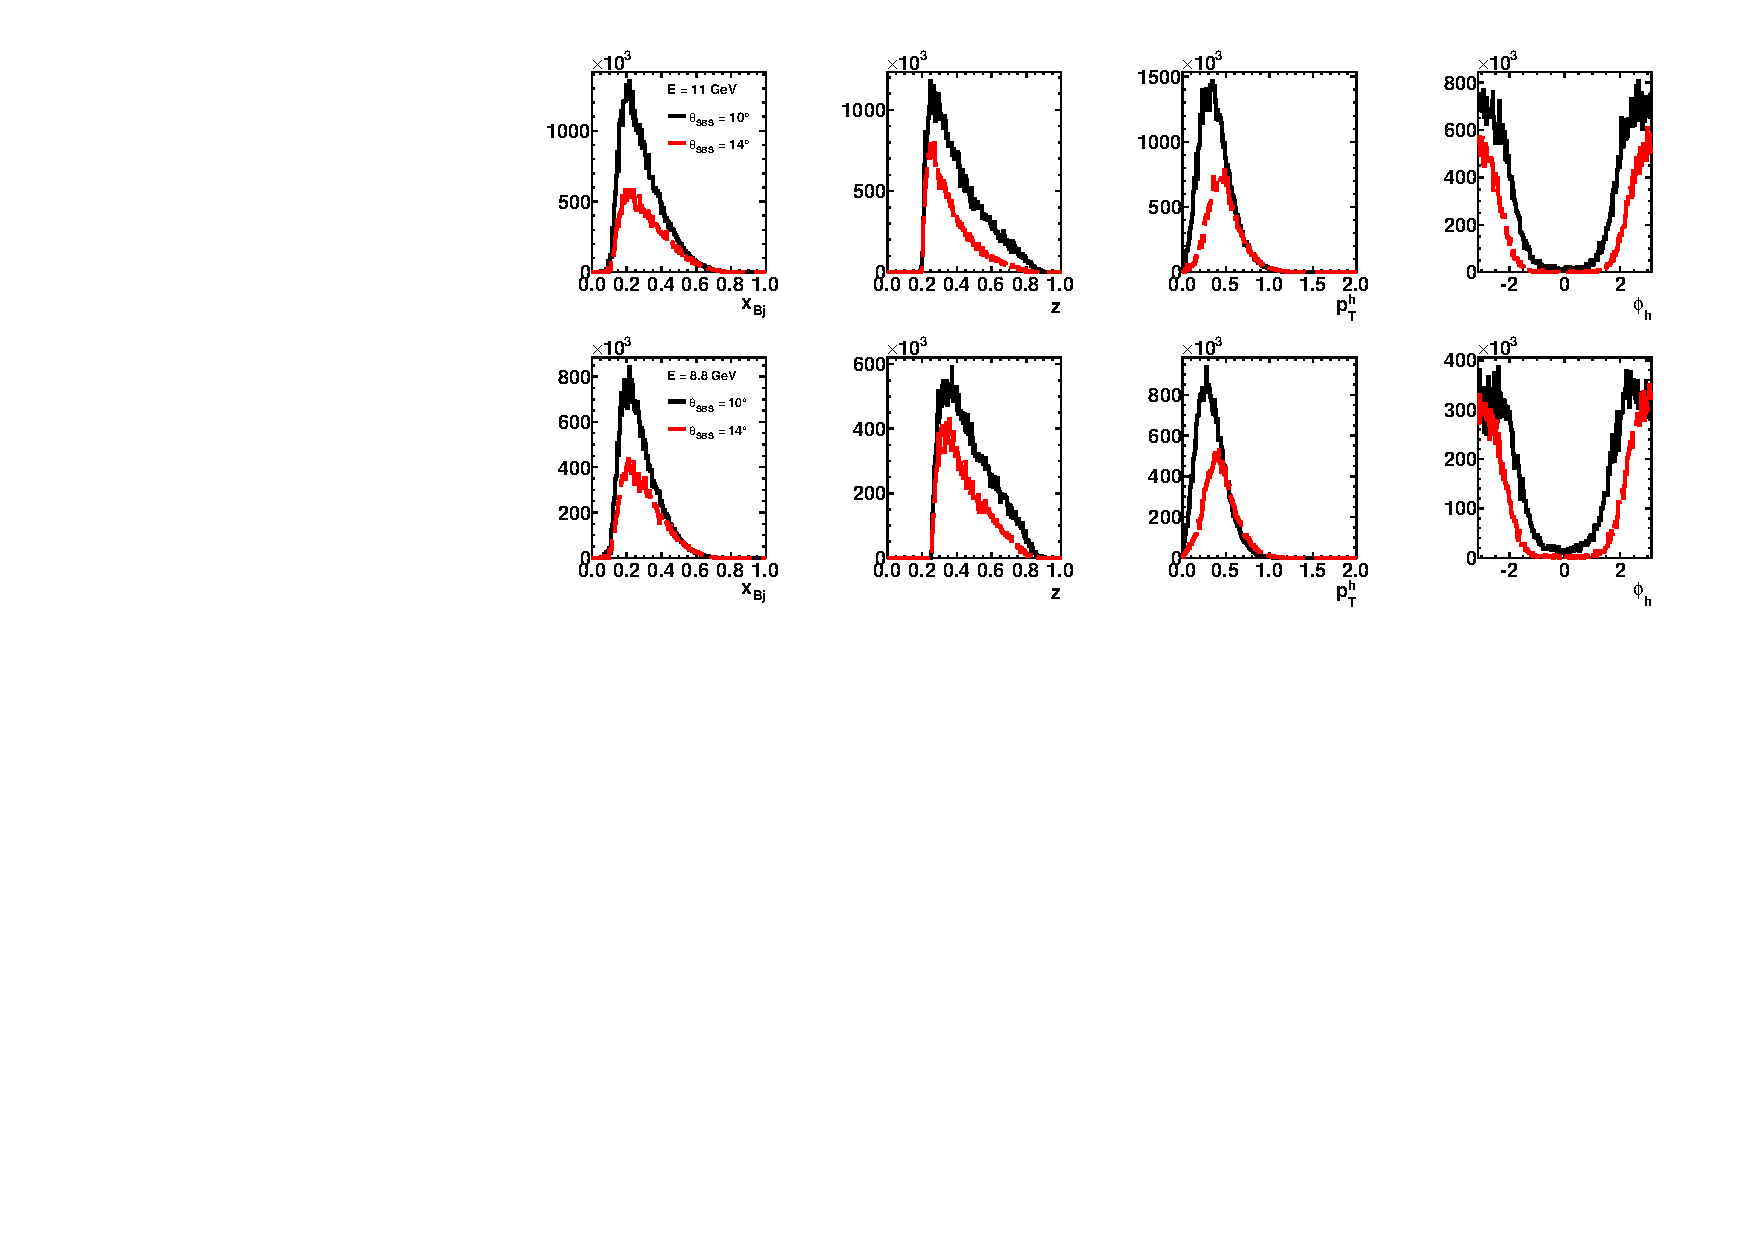
\includegraphics[width=.98\textwidth]{figures/kine14deg10deg_comparison.pdf}
  \end{center}
  \caption{\label{kine14_10_1D} Expected distributions of the kinematic variables $x$, $z$, $p_T^h$ and $\phi_h$ (from left to right) in $^3He(e,e'\pi^+)X$, for $E = 11$ GeV (top row) and $E = 8.8$ GeV (bottom row). Black solid (red dashed) lines are for $\theta_{SBS} = 10^\circ (14^\circ)$. The histograms are normalized so that the vertical axis corresponds to the total number of $^3He(e,e'\pi^+)X$ events in the beam time allocated to the configuration in question.}
\end{figure}
Figure~\ref{kine14_10_1D} shows the projected SIDIS $^3He(e,e'\pi^+)X$ yield as a function of the kinematic variables $x$, $z$, $p_T^h$ and $\phi_h$ for each of the four beam energy/SBS angle configurations. The ten-degree setting exhibits higher event rates at low $x$ and low $p_T^h$ values and greater $\phi_h$ coverage than the 14-degree setting. On the other hand, for $x \gtrsim 0.5$ and $p_T^h \gtrsim 0.6$ GeV, the yield for the 14-degree setting equals or exceeds that of the 10-degree setting. In both settings, the $\phi_h$ coverage is peaked near $\phi_h \approx \pm \pi$, averages about half of 2$\pi$, and increases at low $p_T^h$/high $x$ values. 

\begin{figure}[h]
  \begin{center}
    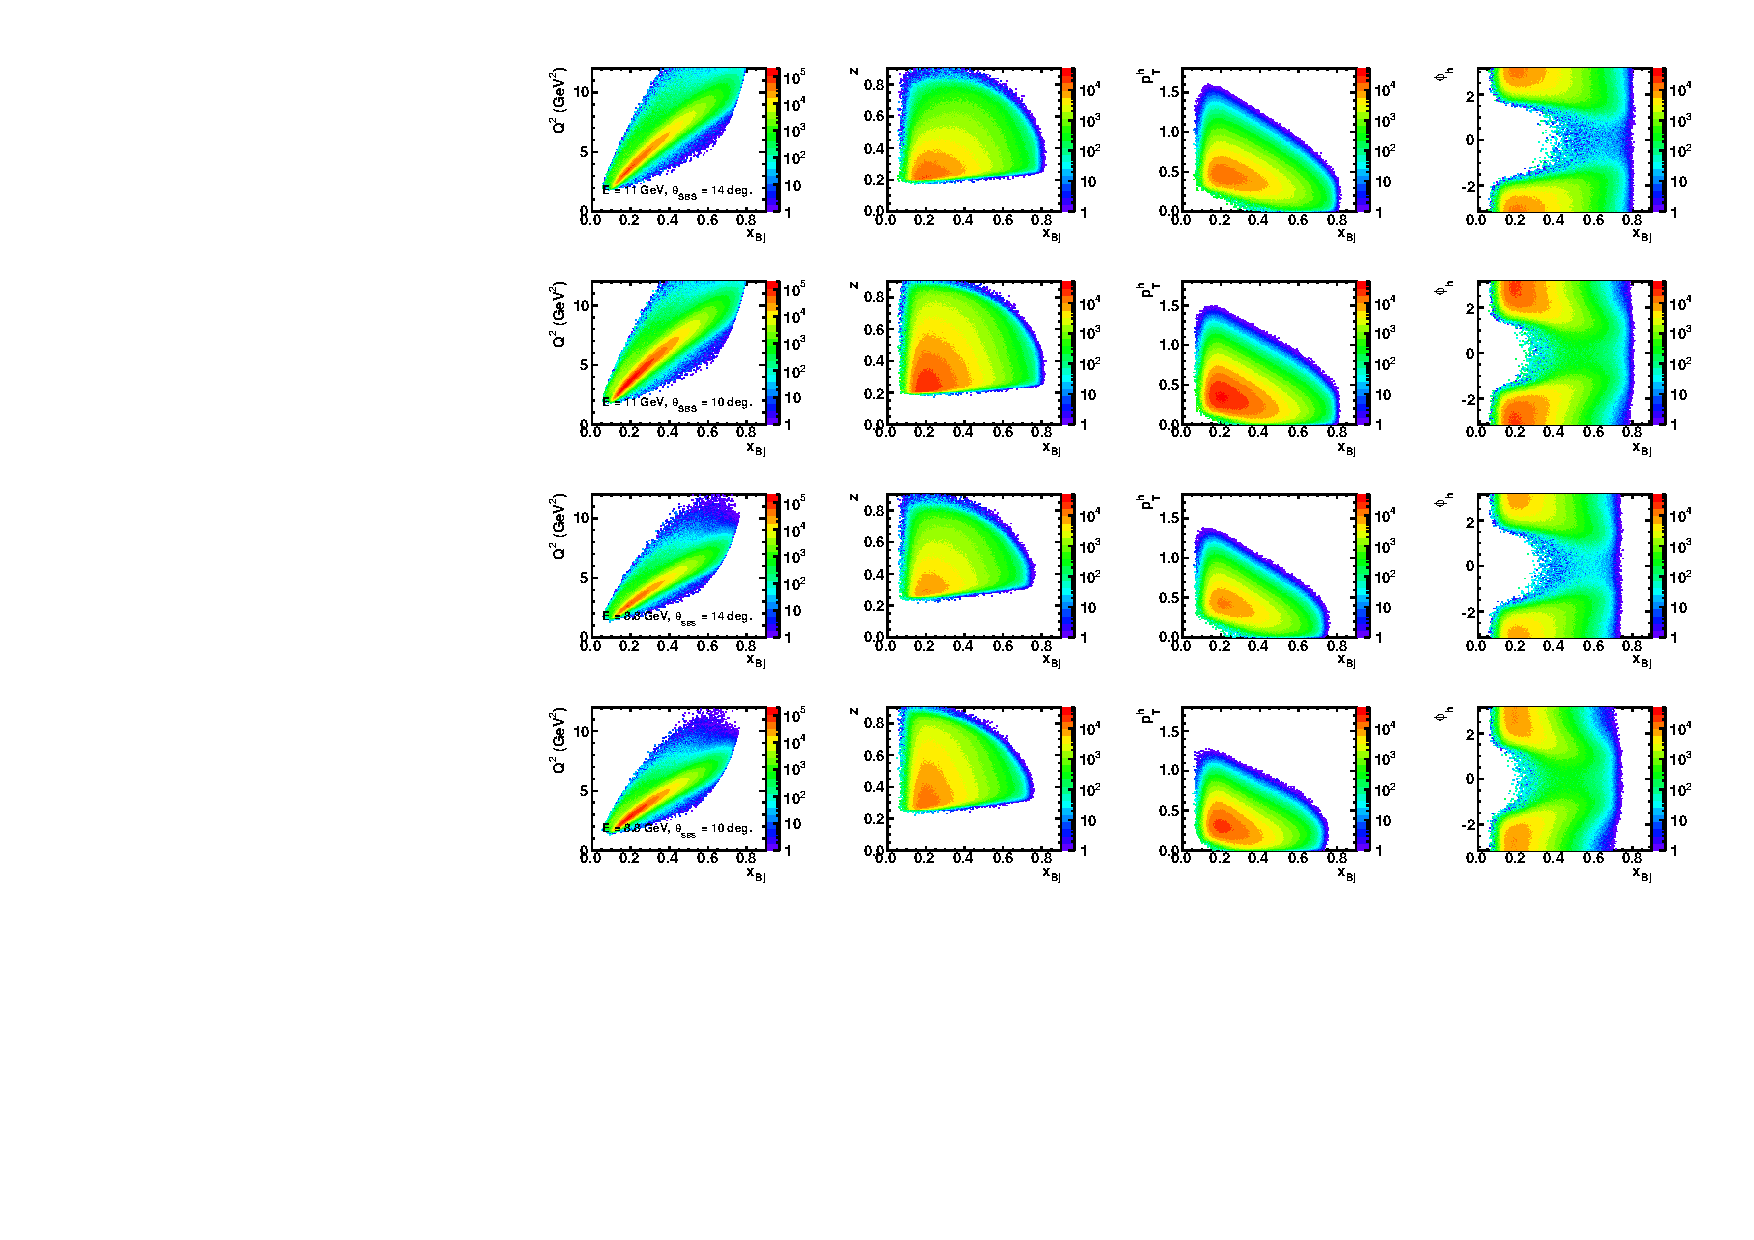
\includegraphics[width=0.98\textwidth]{figures/kine14deg10deg_2Dcomparison.pdf}
  \end{center}
  \caption{\label{kine14_10_2D} SIDIS phase space coverage of the four proposed experiment configurations for the $^3He(e,e'\pi^+)X$ channel. From left to right: $Q^2$, $z$, $p_T^h$ and $\phi_h$ vs $x$. From top to bottom: $E = 11$ GeV, $\theta_{SBS} = 14^\circ$, $E = 11$ GeV, $\theta_{SBS}=10^\circ$, $E = 8.8$ GeV, $\theta_{SBS}=14^\circ$, and $E = 8.8$ GeV, $\theta_{SBS}=10^\circ$. Color scale corresponds to the expected total number of events.}
\end{figure}
Figure~\ref{kine14_10_2D} shows the coverages of the SIDIS kinematic variables $Q^2$, $z$, $p_T^h$ and $\phi_h$ as a function of $x$ in each of the four proposed energy/angle combinations. The color scale of the plots corresponds to the expected total number of $^3He(e,e'\pi^+)X$ events in each bin. $Q^2$ is strongly correlated with $x$ as a consequence of the large horizontal/vertical aspect ratio of the BigBite magnet gap. Due to the large momentum acceptance of both spectrometers, the $z$ and $x$ acceptances are largely uncorrelated, leading to a wide, independent range of $x$ and $z$ within a single angle/beam energy setting. The correlation between the momentum transfer direction and $x$ leads to a weak negative correlation between $p_T^h$ and $x$. The $\phi_h$ coverage increases with $x$ for the same reason.
\subsection{Event Rates}
\paragraph{}
%\subsubsection{Event rates and projected statistics}
\begin{table}[h]
  \caption{\label{RateTable} Expected total SIDIS $^3He(e,e'h)X$ event rates passing all SIDIS kinematic cuts: $Q^2 \ge 1$ GeV$^2$, $W \ge 2$ GeV, $M_X \ge 1.5$ GeV, $y \le 0.9$, $P_h \ge 2$ GeV, $p_e \ge 1$ GeV.}
  \begin{center}
    \begin{tabular}{cccccc}
      \hline \hline
      Channel & $E = 11$ GeV & $E = 11$ GeV & $E = 8.8$ GeV & $E=8.8$ GeV \\ 
      & $\theta_{SBS} = 14^\circ$ & $\theta_{SBS}=10^\circ$ & $\theta_{SBS} = 14^\circ$ & $\theta_{SBS} = 10^\circ$ \\ \hline 
      $^3He(e,e'\pi^+)X$ rate (Hz) & 35.5 & 69.9 & 47.1 & 78.3 \\ 
      $^3He(e,e'\pi^-)X$ rate (Hz) & 23.4 & 43.8 & 28.8 & 45.7 \\
      $^3He(e,e'\pi^0)X$ rate (Hz) & 4.8 & 11.1 & 6.4 & 11.0 \\
      $^3He(e,e'K^+)X$ rate (Hz) & 5.8 & 12.6 & 8.7 & 15.2 \\
      $^3He(e,e'K^-)X$ rate (Hz) & 1.1 & 2.4 & 1.4 & 2.4 \\ \hline \hline 
    \end{tabular}
  \end{center}
\end{table}
Table~\ref{RateTable} shows the total SIDIS event rates for the five hadron species after applying kinematic cuts to select the SIDIS reaction in the current fragmentation region. Although the $\pi^0$ production rate is similar to the charged pion production rates\footnote{The $\pi^0$ fragmentation functions are assumed to be averages of $\pi^+$ and $\pi^-$ (isospin symmetry assumption).}, the SBS acceptance for $\pi^0$s is further reduced relative to the charged pion acceptance by the requirement that both $\pi^0$ decay photons are detected with a minimum separation of one pixel.
%\subsubsection{Extraction of Neutron Asymmetries from $^3$He}
\subsection{Projected Statistical Uncertainties in $A_{1h}^n(x,z)$}
\paragraph{}
The experimentally observed double-spin asymmetry $A_{LL,h}^{exp}$ for hadron $h$ on $^3$He is approximately related to the longitudinal virtual photon asymmetry by:
\begin{eqnarray}
  A_{LL,h}^{exp} &=& P_B P_T A_{LL,h}^{^3He} = P_B P_T \mathcal{P}_{kin} A_{1h}^{^3He} = P_B P_T \mathcal{P}_{kin} \left[P_n f_n A_{1h}^n + P_p f_p A_{1h}^p \right], \label{asymextractformula}
\end{eqnarray}
where $P_B$ and $P_T$ are the beam and target polarizations, $P_n = 0.86_{-0.02}^{+0.036}$ and $P_p = -0.028_{-0.004}^{+0.009}$ are the neutron and proton effective polarizations in $^3$He, $f_{n/p}$ is the ``dilution'' factor representing the fraction of the total $^3$He SIDIS cross section carried by the neutron/protons, and $\mathcal{P}_{kin}$ is the kinematic factor appearing in Eqn.~\eqref{Eq:pkin}. This effective polarization approximation has been used for the extraction of neutron asymmetries from measured $^3$He asymmetries by a number of previous experiments studying DIS on polarized $^3$He targets~\cite{E06010_AUT_PRL,E06010_ALT_PRL,A1N_PRL}. The experimentally observed asymmetry is defined by the asymmetry in the measured SIDIS yield between events obtained with beam and target polarizations parallel and anti-parallel. Defining $N_+ \equiv N_{++} + N_{--}$ and $N_{-} \equiv N_{+-} + N_{-+}$ as the total SIDIS yields in parallel and anti-parallel conditions, respectively, the observed asymmetry is then defined as:
\begin{eqnarray}
  A_{LL,h}^{exp} &=& \frac{N_+ - N_-}{N_+ + N_-}
\end{eqnarray}
The statistical uncertainty in $A_{LL,h}^{exp}$ is given by 
\begin{eqnarray}
  \Delta A_{LL,h}^{exp} &=& \sqrt{\frac{1-(A_{LL,h}^{exp})^2}{N}}, \label{asym_staterr}
\end{eqnarray}
where $N \equiv N_+ + N_-$ is the total number of events. The projected uncertainty in $A_{1h}^n$ for each $(x,z)$ bin was estimated from equations~\eqref{asym_staterr} and \eqref{asymextractformula}. For the ratio $R = \sigma_L/\sigma_T$ that enters the kinematic factor $\mathcal{P}_{kin}$ of equation \eqref{Eq:pkin}, the SLAC R1998 parametrization of inclusive DIS data was used~\cite{SLAC_R1998}, which implies the assumption, in the absence of data for $R$ in SIDIS, that $R_{SIDIS} = R_{DIS}$. In the estimation of $\Delta A_{1h}^n$ for this proposal, the small $A_{1h}^p$ correction due to the small but non-zero proton polarization in $^3$He was neglected. This correction will be well-constrained by existing data from HERMES as well as from future JLab measurements in CLAS12, and its contribution to the systematic uncertainty in $A_{1n}^n$ will be small.

For the analysis of projected physics results, Monte-Carlo generated SIDIS events passing all cuts were subdivided into a two-dimensional rectangular grid of $(x,z)$ bins in the range $(0.1 \le x \le 0.8, 0.2 \le z \le 0.8)$ with bin widths of $(\Delta x, \Delta z) = (0.1, 0.1)$. In each bin, the total number of events and the weighted-average kinematics $<x>$, $<Q^2>$, $<z>$ and $<p_T^h>$ were calculated as well as the kinematic factor $<\mathcal{P}_{kin}>$ and the dilution factor $f_n$. The uncertainty $\Delta A_{1h}^n$ was then calculated in each bin using 
\begin{eqnarray}
  \Delta A_{1h}^n &=& \frac{1}{P_BP_T f_n P_n \mathcal{P}_{kin}\sqrt{N}}\label{da1nh}, 
\end{eqnarray}
where again the small $A_{1h}^p$ correction has been neglected. 
\begin{figure}[h]
  \begin{center}
    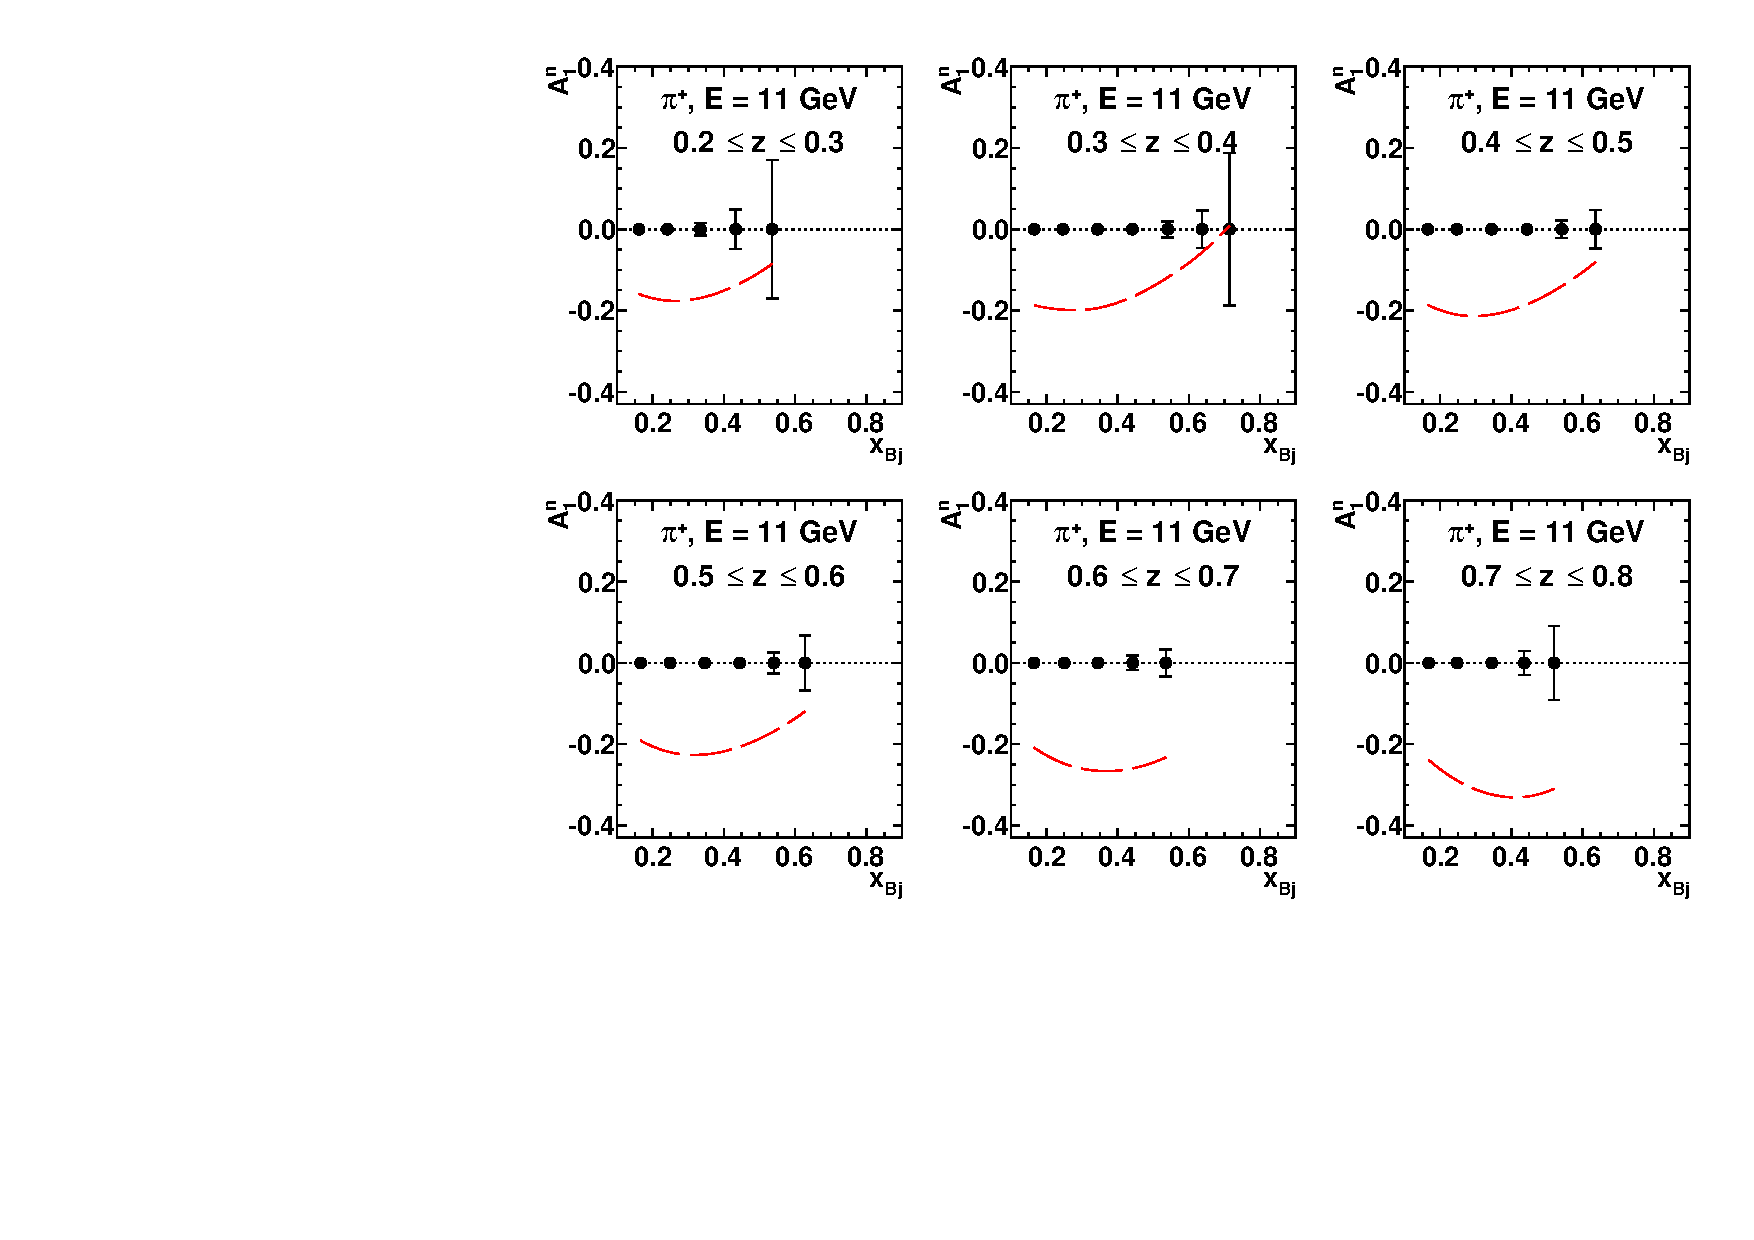
\includegraphics[width=.98\textwidth]{figures/A1n_vs_x_E11_pip.pdf}
  \end{center}
  \caption{\label{A1n_pip_11gev.txt} Projected uncertainties in $A_1^{n,\pi^+}(x,z)$ from combined 11 GeV running at both SBS angle settings, compared to the predictions of the recent NLO global QCD analysis of DSSV~\cite{deFlorian:2014yva}}
\end{figure}


\subsection{Comparison to Existing Data}
\subsection{Comparison to Other Approved Experiments}

